\documentclass[aspectratio=169,11pt]{beamer}
\usepackage{tikz}
\graphicspath{{/Users/dehmelf/Downloads/unified-aa-talk-assets/}{unified-aa-talk-assets/}}
\usetikzlibrary{arrows.meta,overlay-beamer-styles}
\usefonttheme{serif}
\usepackage{newtxtext,newtxmath}
\setbeamertemplate{navigation symbols}{}
\setbeamersize{text margin left=.55cm,text margin right=.55cm}
\setbeamertemplate{frametitle}{\vskip.14cm\hspace*{-.18cm}\Large\color{black}\strut\insertframetitle\par}
\definecolor{GuideBlue}{HTML}{147CA7}
\definecolor{SoftBlue}{HTML}{D9E8F5}
\definecolor{SoftPeach}{HTML}{FCE4D6}
\definecolor{NoteOrange}{HTML}{E85E0D}
\definecolor{SoftGreen}{HTML}{C6E0B4}
\definecolor{Highlight}{HTML}{FFFF00}

\tikzset{
  box/.style={draw, thin, inner sep=5pt, align=center},
  tree/.style={box, fill=SoftBlue, minimum width=1.35cm},
  arrow/.style={-{Stealth[length=2mm]},draw=GuideBlue,semithick},
  callout/.style={box,fill=SoftPeach,draw=NoteOrange},
  conclusion/.style={box,fill=black!8,draw=red,semithick}
}
% Change to \setbeameroption{show notes} to print speaker notes.
\setbeameroption{hide notes}

% Bucket labels run down the rows; each row contains hashed output strings.
\newcommand{\bucketpicture}{%
  \fill[SoftBlue] (7.35,3.35) rectangle (14.55,3.88);
  \fill[SoftGreen!45] (7.35,2.35) rectangle (14.55,2.85);
  \draw (7.35,1.85) rectangle (14.55,3.88);
  \draw (8.5,1.85)--(8.5,3.88);
  \foreach \y in {3.35,2.85,2.35}{\draw (7.35,\y)--(14.55,\y);}
  \node[font=\small] at (7.925,3.615) {Bucket};
  \node[font=\small] at (11.525,3.615) {Output strings};
  \node at (7.925,3.1) {$b_1$};
  \node at (7.925,2.6) {$b_2$};
  \node at (7.925,2.1) {$b_3$};
  \node[anchor=west,font=\ttfamily\scriptsize] at (8.65,3.1)
    {10101011\ldots,\quad 100110100\ldots,\quad\ldots};
  \node[anchor=west,font=\scriptsize] at (8.65,2.6)
    {\texttt{01100101\ldots},\quad {\color{GuideBlue}\large $y^*$},\quad \texttt{11010010\ldots},\quad\ldots};
  \node[anchor=west,font=\ttfamily\scriptsize] at (8.65,2.1)
    {00110101\ldots,\quad 10110100\ldots,\quad\ldots};
}
\newcommand{\beginproofcanvas}{%
  \draw[GuideBlue,densely dotted] (7.08,1.25)--(7.08,4.25);
}

\usetikzlibrary{positioning,calc,decorations.pathreplacing}
\newcommand{\band}[1]{\begin{center}\colorbox{Highlight}{\parbox{.89\linewidth}{\centering\strut #1\strut}}\end{center}}
\newcommand{\takeaway}[1]{\par\medskip\begin{center}\fcolorbox{red}{black!5}{\parbox{.86\linewidth}{\centering #1}}\end{center}}
\newcommand{\credit}[1]{\par\medskip{\scriptsize\color{black!66}#1}}
\newcommand{\E}{\mathbb E}
\newcommand{\Var}{\operatorname{Var}}
\newcommand{\Inf}{\operatorname{Inf}}
\newcommand{\poly}{\operatorname{poly}}
\newcommand{\axisbase}{%
  \draw[arrow] (.25,0)--(13.1,0) node[below left=3pt] {Oracle queries (schematic)};
  \draw[thick] (2.6,-.16)--(2.6,.16);
  \node[align=center,above=6pt] at (2.6,0) {YZ quantum upper bound\\[-1pt]\small Polynomially many suffice};
  \draw[thick] (10.6,-.16)--(10.6,.16);
  \node[align=center,above=6pt] at (10.6,0) {YZ classical lower bound\\[-1pt]\small Exponentially many required};
  \draw[draw=NoteOrange,thick] (1.03,-.12)--(1.03,.12);
  \node[align=center,below=8pt,font=\small,text=NoteOrange] at (1.03,0) {Our fixed\\quantum budget};
}
\begin{document}
\begin{frame}[plain]
\centering
{\LARGE Classical Simulation of Quantum Queries\par}
\medskip
{\large Aaronson--Ambainis, Gibbs Sampling, Hard Sectors and Certified Randomness\par}
\vspace{.85cm}
{Frederick Dehmel, Jason Dong, Ian Loam, Praneel Samal}
\note{The talk starts with one yes-or-no probability and follows two applications of classical query simulation.}
\end{frame}

\begin{frame}{The Aaronson--Ambainis question}
\begin{center}
\begin{tikzpicture}
\node[font=\large] at (2.7,4.8) {Quantum algorithm};
\node[font=\large] at (10.7,4.8) {Classical algorithm};
\node at (2.7,2.2) {\includegraphics[width=4.3cm]{quantum-algorithm.jpg}};
\node at (10.7,2.2) {\includegraphics[width=9cm]{function-machine.jpg}};
\draw[draw=GuideBlue,line width=3.5pt,-{Stealth[length=6mm,width=5mm]}] (5.15,2.2)--(8.1,2.2);
\node[font=\Large] at (6.6,2.9) {simulate?};
\path (0,0) rectangle (13.1,5.15);
\end{tikzpicture}
\end{center}
\note{User-supplied images: https://www.purposegames.com/game/function-machine ; Dreamstime image 262685515, https://www.dreamstime.com/quantum-computing-icon-vector-illustration-flat-outline-cartoon-artificial-intelligence-concept-isolated-premium-image262685515 . Quantum preview watermark retained. Simulation means estimating acceptance probability using classical input queries.}
\end{frame}

\begin{frame}{The Aaronson--Ambainis conjecture (or should we say theorem [Tur26])}
\begin{center}
\begin{tikzpicture}[
 dn/.style={circle,draw=black!35,fill=black!5,minimum size=4.5mm,inner sep=0pt},
 active/.style={circle,draw=GuideBlue,thick,fill=SoftGreen,minimum size=5.5mm,inner sep=0pt}
]
\node[font=\large] at (1.7,4.25) {Quantum algorithm};
\node at (1.7,2.65) {\includegraphics[width=3.0cm]{quantum-algorithm.jpg}};
\node[font=\small] at (1.7,.95) {$Q$ queries};
\draw[arrow,line width=1.2pt] (3.35,2.65)--(4.2,2.65);
\node[font=\large] at (6.4,4.25) {Acceptance polynomial};
\node[align=center] at (6.4,2.85)
 {$\displaystyle p(x)=\sum_{|S|\le 2Q}a_S\prod_{i\in S}x_i$};
\node[font=\small] at (6.4,1.65) {$p(x)=\Pr[\mathrm{accept}\mid x]$};
\node[font=\small] at (6.4,.95) {$0\le p(x)\le 1,\quad\deg p\le 2Q$};
\draw[arrow,line width=1.2pt] (8.6,2.65)--(9.7,2.65);
\node[font=\small] at (9.15,3.15) {simulate?};
\node[font=\large] at (11.5,4.25) {Classical decision tree};
\node[active] (r) at (11.5,3.4) {};
\node[active] (a) at (10.6,2.65) {};
\node[dn] (b) at (12.4,2.65) {};
\foreach \n/\x in {l0/10.15,l1/11.05,l2/11.95,l3/12.85}{\node[dn] (\n) at (\x,1.9) {};}
\foreach \u/\v in {r/b,a/l0,b/l2,b/l3}{\draw[black!30] (\u)--(\v);}
\draw[arrow,very thick] (r)--(a);
\draw[arrow,very thick] (a)--(l1);
\node[active] at (11.05,1.9) {};
\node[font=\small] at (11.5,.95) {Estimate $p(x)$};
\path (0,.5) rectangle (13.5,4.65);
\end{tikzpicture}
\end{center}
\credit{Aaronson--Ambainis (2014). Proved in 2026 by Turturean.}
\note{On Boolean inputs, a Q-query quantum algorithm has a bounded multilinear acceptance polynomial of degree at most 2Q. This represents its acceptance probability, not its full quantum state. The scalar AA simulation statement gives a classical decision tree with query cost polynomial in Q and inverse accuracy and failure parameters, approximating p on most uniformly random inputs. The next lemma explains how to choose its queries.}
\end{frame}

\begin{frame}{Representing a quantum algorithm by a polynomial}

Fix a quantum algorithm making $Q$ queries to
$x\in\{0,1\}^N$.

\begin{enumerate}[<+->]
  \item \textbf{Amplitudes are low-degree polynomials.}\\
  Each query increases the degree by at most one.

  After $Q$ queries, each amplitude has degree at most $Q$.

  \medskip
  \item \textbf{Probabilities square the amplitudes.}
  \[
    p(x):=\Pr[A^x=1]
      =\sum_{z:\,\mathrm{accept}} |a_z(x)|^2.
  \]
  Therefore
  \[
    \boxed{\deg(p)\le 2Q,\qquad 0\le p(x)\le1.}
  \]

  \item \textbf{Apply AA to this polynomial.}\\
  If $p$ still has substantial variance, AA guarantees
  an influential input bit.
  Query that bit and repeat.
\end{enumerate}

\medskip
\uncover<3->{%
Once the remaining variance is small, estimate $p(x)$
by its conditional mean.}

\end{frame}


% \begin{frame}{Two uses of classical query simulation}
% \band{How much can a classical algorithm learn from a few input queries?}
% \begin{center}
% \begin{tikzpicture}
% \node[box,fill=SoftBlue] (aa) {Estimate a quantum acceptance probability};
% \node[box,fill=SoftPeach,text width=4.7cm] (g) at (-3.35,-1.65) {Correlated inputs\\High-temperature Gibbs simulation};
% \node[box,fill=SoftGreen,text width=4.7cm] (r) at (3.35,-1.65) {Long outputs\\Certified randomness from hashing};
% \draw[arrow] (aa.south)--(g.north);
% \draw[arrow] (aa.south)--(r.north);
% \end{tikzpicture}
% \end{center}
% \note{The Gibbs theorem and the randomness proof are separate. Both use local estimation, and the randomness section returns to a uniform random oracle.}
% \end{frame}
\begin{frame}{The influential-bit lemma}
\band{A varying low-degree function has at least one bit that matters.}

\begin{center}
\begin{tikzpicture}[node distance=9mm]
  \node[box,fill=SoftBlue,text width=3.1cm] (f)
    {Restricted function $p|_{\rho}$};

  \uncover<2->{%
    \node[align=center,right=of f] (lemma)
      {\includegraphics[width=2.4cm]{influential-bit-lemma.jpg}\\
       Influential-bit lemma};
    \draw[arrow] (f)--(lemma);
  }

  \uncover<3->{%
    \node[box,fill=SoftGreen,text width=3.0cm,right=of lemma] (i)
      {Coordinate $i$ with substantial influence};
    \draw[arrow] (lemma)--(i);
  }
\end{tikzpicture}
\end{center}

\uncover<4->{%
  \takeaway{Influence measures how much $p$ changes, on average,
  when one coordinate is flipped.}
}

\note{This is the qualitative content of the
Aaronson--Ambainis influential-bit theorem. Exact exponents
are not needed for the decision-tree picture.}
\end{frame}
\begin{frame}{The influential-bit lemma}
\band{A varying low-degree function has at least one bit that matters.}

\begin{center}
\begin{tikzpicture}[node distance=9mm]
  \node[box,fill=SoftBlue,text width=3.1cm] (f)
    {Restricted function $p|_{\rho}$};

  \uncover<2->{%
    \node[align=center,right=of f] (lemma)
      {\includegraphics[width=2.4cm]{influential-bit-lemma.jpg}\\
       Influential-bit lemma};
    \draw[arrow] (f)--(lemma);
  }

  \uncover<3->{%
    \node[box,fill=SoftGreen,text width=3.0cm,right=of lemma] (i)
      {Coordinate $i$ with substantial influence};
    \draw[arrow] (lemma)--(i);
  }
\end{tikzpicture}
\end{center}

\uncover<4->{%
  \takeaway{Influence measures how much $p$ changes, on average,
  when one coordinate is flipped.}
}

\note{This is the qualitative content of the
Aaronson--Ambainis influential-bit theorem. Exact exponents
are not needed for the decision-tree picture.}
\end{frame}


\begin{frame}{Query the lemma along the path}
\begin{center}
\begin{tikzpicture}[
 dn/.style={
   circle,draw=black!35,fill=black!5,
   minimum size=5mm,inner sep=0pt
 },
 active/.style={
   circle,draw=GuideBlue,thick,fill=SoftGreen,
   minimum size=6mm,inner sep=0pt
 },
 edge/.style={draw=black!25,thin},
 route/.style={
   draw=GuideBlue,very thick,-{Stealth[length=2mm]}
 },
 call/.style={
   draw=NoteOrange,densely dashed,-{Stealth[length=2mm]}
 }
]

% Full tree.
\node[dn] (r)  at (4,4.15) {};
\node[dn] (a)  at (2,2.95) {};
\node[dn] (b)  at (6,2.95) {};
\node[dn] (aa) at (1,1.75) {};
\node[dn] (ab) at (3,1.75) {};
\node[dn] (ba) at (5,1.75) {};
\node[dn] (bb) at (7,1.75) {};

\node[dn] (leafA) at (.5,.55) {};
\node[dn] (leafB) at (1.5,.55) {};
\node[dn] (leafC) at (2.5,.55) {};
\node[dn] (leafD) at (3.5,.55) {};
\node[dn] (leafE) at (4.5,.55) {};
\node[dn] (leafF) at (5.5,.55) {};
\node[dn] (leafG) at (6.5,.55) {};
\node[dn] (leafH) at (7.5,.55) {};

% Explicit edges avoid the earlier misdirected edge.
\draw[edge] (r)--(a);
\draw[edge] (r)--(b);
\draw[edge] (a)--(aa);
\draw[edge] (a)--(ab);
\draw[edge] (b)--(ba);
\draw[edge] (b)--(bb);
\draw[edge] (aa)--(leafA);
\draw[edge] (aa)--(leafB);
\draw[edge] (ab)--(leafC);
\draw[edge] (ab)--(leafD);
\draw[edge] (ba)--(leafE);
\draw[edge] (ba)--(leafF);
\draw[edge] (bb)--(leafG);
\draw[edge] (bb)--(leafH);

% 1: Start at the root.
\node[active] at (r.center) {};

% 2: Call IB at the root.
\uncover<2->{%
  \node[inner sep=0pt] (ib0) at (6.5,4.15)
    {\includegraphics[width=1.15cm]{influential-bit-lemma.jpg}};
  \draw[call] (r.east)--
    node[above,font=\scriptsize] {IB $\to i$}
    (ib0.west);
}

% 3: Query i and move down.
\uncover<3->{%
  \draw[route] (r)--
    node[left,font=\scriptsize] {$x_i=0$} (a);
  \node[active] at (a.center) {};
}

% 4: Call IB at the next node.
\uncover<4->{%
  \node[inner sep=0pt] (ib1) at (.45,2.95)
    {\includegraphics[width=1.15cm]{influential-bit-lemma.jpg}};
  \draw[call] (a.west)--
    node[above,font=\scriptsize] {IB $\to j$}
    (ib1.east);
}

% 5: Query j and move down.
\uncover<5->{%
  \draw[route] (a)--
    node[right,font=\scriptsize] {$x_j=1$} (ab);
  \node[active] at (ab.center) {};
}

% 6: Call IB once more.
\uncover<6->{%
  \node[inner sep=0pt] (ib2) at (4.05,1.75)
    {\includegraphics[width=.95cm]{influential-bit-lemma.jpg}};
  \draw[call] (ab.east)--(ib2.west);
  \node[font=\scriptsize] at (4.05,1.16)
    {IB $\to k$};
}

% 7: Query k and move to the leaf.
\uncover<7->{%
  \draw[route] (ab)--
    node[left,font=\scriptsize] {$x_k=0$} (leafC);
  \node[active] at (leafC.center) {};
}

% Residual variance appears after each query.
\node[font=\scriptsize,align=center] at (11,4.85)
  {Residual variance\\averaged over paths};
\node at (11,4.15)
  {$\Var(p(X))$};

\uncover<3->{%
  \node[font=\Large] at (11,3.55)
    {\rotatebox{90}{$\le$}};
  \node at (11,2.95)
    {$\mathbb E[\Var(p(X)\mid\rho_1)]$};
}

\uncover<5->{%
  \node[font=\Large] at (11,2.35)
    {\rotatebox{90}{$\le$}};
  \node at (11,1.75)
    {$\mathbb E[\Var(p(X)\mid\rho_2)]$};
}

\uncover<7->{%
  \node[font=\Large] at (11,1.15)
    {\rotatebox{90}{$\le$}};
  \node at (11,.55)
    {$\mathbb E[\Var(p(X)\mid\rho_3)]$};
}

% Fixed layout across overlays; no visible bounding-box line.
\pgfresetboundingbox
\pgfpathrectangle
  {\pgfpointxy{-.25}{.1}}
  {\pgfpointxy{14.05}{5.05}}
\pgfusepath{use as bounding box}

\end{tikzpicture}
\end{center}

\note{Each IB call and each move occupies a separate overlay.
Here rho_k is the random restriction after k queries.
Residual variance is nonincreasing in expectation over all
paths, by total variance; it need not decrease on each
individual path. The displayed depth-three tree is schematic.
Image: https://www.purposegames.com/game/function-machine .}
\end{frame}

% \begin{frame}{What routing has to produce}
% \band{A bichromatic pair, a face $T\subseteq\Delta(x,y)$ that is monochromatic for $x$, and a point of $A$ close to $y$.}
% \begin{center}
% \begin{tikzpicture}[every node/.style={font=\scriptsize}]
%   \fill[SoftGreen!60] (-1.4,-1.0) -- (-1.4,2.6)
%      .. controls (1.2,2.85) and (4.2,2.8) .. (6.0,2.7)
%      .. controls (7.0,2.6) and (7.2,1.9) .. (7.25,1.0)
%      .. controls (7.3,0.0) and (6.6,-0.7) .. (5.3,-1.0) -- cycle;
%   \draw[SoftGreen!50!black,line width=.8pt] (-1.4,2.6)
%      .. controls (1.2,2.85) and (4.2,2.8) .. (6.0,2.7)
%      .. controls (7.0,2.6) and (7.2,1.9) .. (7.25,1.0)
%      .. controls (7.3,0.0) and (6.6,-0.7) .. (5.3,-1.0);
%   \node[font=\small,SoftGreen!45!black] at (-0.9,2.0) {$A$};
%   \draw[GuideBlue,fill=SoftGreen,line width=.9pt] (3.0,1.95)--(4.35,1.0)--(3.0,.05)--(1.65,1.0)--cycle;
%   \draw[GuideBlue,densely dotted,line width=.9pt] (7.7,2.55)--(11.05,1.0)--(7.7,-.55)--(4.35,1.0)--cycle;
%   \fill (1.65,1.0) circle (1.7pt);  \node[below left] at (1.63,.94) {$x$};
%   \fill (4.35,1.0) circle (1.7pt);
%   \draw[black!45,line width=.6pt] (4.32,.95)--(4.15,.5);
%   \node[font=\tiny,anchor=north] at (4.1,.45) {$x\oplus T$};
%   \fill (11.05,1.0) circle (1.7pt); \node[right] at (11.1,1.0) {$y$};
%   \fill[GuideBlue] (6.3,1.55) circle (1.9pt); \node[right,GuideBlue] at (6.38,1.55) {$z$};
%   \draw[arrow,GuideBlue] (10.9,.85) .. controls (9.5,.6) and (7.6,1.2) .. (6.45,1.5);
%   \node[font=\tiny] at (2.65,2.15) {$\mathrm{cube}(x,x\oplus T)\subseteq A$};
%   \node[font=\tiny] at (7.7,-.7) {$\mathrm{cube}(x\oplus T,y)$};
% \end{tikzpicture}
% \end{center}
% {\small\textbf{(a)} $z\in A\cap\mathrm{cube}(x\oplus T,y)$: $z$ agrees with $y$ outside $\Delta(x,y)\setminus T$, so the route walks only in the unfrozen directions.}
% \par\smallskip
% {\small\textbf{(b)} for every $i$: $\Pr\big[x\in A,\,y\notin A,\,z_i\neq y_i\big]\le\tfrac14\operatorname{Inf}_i(A)$.}

% \credit{Blanc, Docter, Strassle and Tan, \S2.4 (Lemma 2.10, Fig.~3).}

% \end{frame}


% \begin{frame}{Routing links certificates to influence}
% \band{Freeze the heavy coordinates of $y$'s certificate, and walk only on the light ones.}
% \begin{center}
% \begin{tikzpicture}[every node/.style={font=\scriptsize},
%   hc/.style={draw=SoftPeach!55!black,fill=SoftPeach,minimum width=.8cm,minimum height=.62cm,inner sep=0pt},
%   lc/.style={draw=black!30,fill=white,minimum width=.8cm,minimum height=.62cm,inner sep=0pt}]
%   \foreach \k in {0,1,2} {\node[hc] at (\k*0.8+0.4,1.0) {};}
%   \foreach \k in {0,1,2,3} {\node[lc] at (2.8+\k*0.8+0.4,1.0) {};}
%   \draw[black!35,densely dashed] (2.4,.62)--(2.4,1.38);
%   \node[font=\tiny,anchor=south,align=center] at (1.2,1.42) {$T$ frozen: $\lambda_y(i)>\tau$\\$z$ keeps $y$'s values};
%   \node[font=\tiny,anchor=south,align=center] at (4.4,1.42) {free: $\lambda_y(i)\le\tau$\\the walk uses these};
%   \draw[arrow,GuideBlue] (2.55,.42)--(5.55,.42);
%   \node[font=\tiny,GuideBlue,anchor=north] at (4.05,.35) {$\ge 1/\tau$ steps};
%   \fill (0.0,1.0) circle (1.7pt); \node[left] at (-0.08,1.0) {$y$};
%   \fill[GuideBlue] (5.75,1.0) circle (1.9pt); \node[right,GuideBlue] at (5.83,1.0) {$z\in A$};
% \end{tikzpicture}
% \end{center}
% {\small Since $y\notin A$ and $z\in A$, the certificate of $y$ charges the route, $\lambda_y(\Delta(y,z))\ge 1$, and every step is cheap: $\operatorname{dist}(y,z)\ge 1/\tau$.}
% \uncover<2->{\small Markov with the measure $\lambda_x$ gives $\lambda_x(T)\le\operatorname{overlap}/\tau$; with $\tau=\operatorname{overlap}$ this is below $1$, so $T$ is a face and routing applies.}
% \uncover<3->{\takeaway{Overlap buys distance: $\operatorname{dist}(y,z)\ge 1/\operatorname{overlap}$, which is the all-pairs inequality; Cauchy--Schwarz then gives the certificate--influence inequality.}}
% \credit{Blanc, Docter, Strassle and Tan, \S\S2.3--2.4.2 and \S6 (Fig.~4).}
% \note{Fractional certificates for opposite labels need not share a heavy coordinate, so literal intersection fails; the overlap is what is left of it.}
% \end{frame}


% \begin{frame}{The crux is antipodal: a walk that never leaves $A$}
% \band{$y$ is the antipode of $x$ inside $\mathrm{cube}(x,y)$: route $x$ close to $\bar x$, subcube by subcube.}
% {\small\textbf{(a)} $z\in\mathrm{cube}(x\oplus T,\bar x)$ \qquad \textbf{(b)} $\Pr\big[x\in A,\,z_i\neq\bar x_i\big]\le\tfrac12\operatorname{Inf}_i(A)$; the two $\tfrac12$'s give the $\tfrac14$.}
% \begin{center}
% \begin{tikzpicture}[every node/.style={font=\scriptsize},
%   w/.style={draw=black!30,fill=white,rounded corners=2pt,inner sep=3pt,font=\ttfamily\small}]
%   \node[w] (w0) at (0.9,1.15) {\texttt{11001}};
%   \node[w] (w1) at (4.0,1.15) {\texttt{11}\textcolor{red!70!black}{\texttt{1}}\texttt{01}};
%   \node[w] (w2) at (7.1,1.15) {\texttt{111}\textcolor{red!70!black}{\texttt{1}}\texttt{1}};
%   \node[w] (w3) at (10.2,1.15) {\texttt{1111}\textcolor{red!70!black}{\texttt{0}}};
%   \draw[arrow] (w0)--node[above,font=\tiny]{$3$}(w1);
%   \draw[arrow] (w1)--node[above,font=\tiny]{$4$}(w2);
%   \draw[arrow] (w2)--node[above,font=\tiny]{$5$}(w3);
%   \node[font=\tiny,anchor=south] at (0.9,1.6) {$x$};
%   \node[font=\tiny,anchor=south] at (10.2,1.6) {$z$};
%   \node[draw=red!70!black,fill=white,rounded corners=2pt,minimum width=2.7cm,minimum height=.5cm,inner sep=2pt,font=\scriptsize,text=red!70!black] at (1.9,0.05) {$w\oplus i\notin A$};
%   \draw[red!70!black,densely dashed,-{Latex[length=1.4mm]}] (0.8,.9)--(1.5,.32);
%   \node[font=\tiny,red!70!black,anchor=west] at (3.4,.05) {skip $i=1,2$, and charge each edge};
% \end{tikzpicture}
% \end{center}
% \uncover<2->{\small Each skipped flip is charged to the bichromatic edge $\{w,w\oplus i\}$ it would have crossed, and every such edge is charged once: $\#\{x\in A:z_i\neq\bar x_i\}=\#\{x\in A:x\oplus i\notin A\}$, which is (b).}
% \uncover<3->{\takeaway{The canonical-path proof of Poincar\'e, with exits skipped and charged: $z$ and $\bar x$ differ exactly in the skipped coordinates.}}
% \credit{Blanc, Docter, Strassle and Tan, \S2.5.1 (Proposition 2.12).}
% \note{The walk is a permutation of A. Unlike the Poincare walk it never leaves A, and it charges every skipped flip, not only the first.}
% \end{frame}


% \begin{frame}{Faces break the sweep, so average with signs}
% \band{A face demands a flip the sweep may skip; a signed average over all permutations repairs it.}
% \begin{columns}[T]
% \begin{column}{0.38\textwidth}
% \centering
% \begin{tikzpicture}[every node/.style={font=\scriptsize},yshift=2mm]
%   \draw[black!25] (0,0) rectangle (3,2.6);
%   \fill (0,2.6) circle (1.8pt); \fill (3,2.6) circle (1.8pt);
%   \fill (0,0) circle (1.8pt); \fill (3,0) circle (1.8pt);
%   \node[font=\tiny,anchor=north west] at (0.12,2.48) {$x$};
%   \node[font=\tiny,anchor=north east] at (2.88,2.48) {$x\oplus i$};
%   \node[font=\tiny,anchor=south west] at (0.12,0.12) {$x\oplus j$};
%   \node[font=\tiny,anchor=south east] at (2.88,0.12) {$x\oplus\{i,j\}$};
%   \node[GuideBlue,font=\tiny,anchor=east] at (-0.12,2.6) {$1$};
%   \node[GuideBlue,font=\tiny,anchor=west] at (3.12,2.6) {$-\zeta_i$};
%   \node[GuideBlue,font=\tiny,anchor=east] at (-0.12,0) {$-\zeta_j$};
%   \node[GuideBlue,font=\tiny,anchor=west] at (3.12,0) {$\zeta_i\zeta_j$};
%   \node[font=\tiny,anchor=north,text width=4cm,align=center] at (1.5,-0.3) {rows of $M$ on the face $T(x)=\{i,j\}$};
% \end{tikzpicture}
% \end{column}
% \begin{column}{0.60\textwidth}
% \small
% The matrix $M[x,z]=\prod_{i}\zeta_i^{\,1[x_i=z_i]}$ records agreement, and
% \[ \det M=\sum_{\pi}\operatorname{sign}(\pi)\prod_{i}\zeta_i^{\operatorname{err}_i(\pi)} \]
% sums over all permutations of $A$.
% \uncover<2->{A monomial survives with $k_i/2^n\le\tfrac12\operatorname{Inf}_i(A)$ for every $i$, and $\det M_T$ keeps only the face-respecting $\pi$, with $\operatorname{minimal}(\det M_T)=\operatorname{minimal}(\det M)$: a face row is the signed combination on the left.}
% \end{column}
% \end{columns}
% \uncover<3->{\takeaway{A face-respecting permutation with $\operatorname{err}_i\le k_i$ exists, which is (a) and (b) of the antipodal lemma.}}
% \credit{Blanc, Docter, Strassle and Tan, \S\S2.5.2--2.5.3.}
% \note{Minimal means no monomial is below it in every coordinate. The factors in that signed combination are 1 at $\zeta=0$, so they cannot change which monomials are minimal. The surviving monomial has a nonzero coefficient, so it comes from a permutation with those error counts.}
% \end{frame}

\begin{frame}{What changes under a different distribution of inputs?}
\band{AA assumes a uniform input. Correlated bits can constrain one another.}
\begin{center}
\small
\begin{tabular}{lcl}
uniform cube & $\longrightarrow$ & independent fair bits \\[2pt]
biased product law & $\longrightarrow$ & independence, unequal biases \\[2pt]
fixed-weight slice & $\longrightarrow$ & one global count constraint
\end{tabular}
\end{center}
\begin{center}
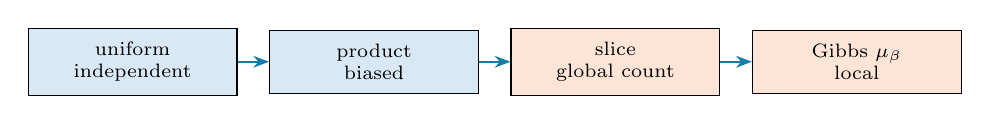
\begin{tikzpicture}[every node/.style={font=\scriptsize}]
\node[box,fill=SoftBlue,text width=2.3cm] (a) {uniform\\independent};
\node[box,fill=SoftBlue,text width=2.3cm,right=4mm of a] (b) {product\\biased};
\node[box,fill=SoftPeach,text width=2.3cm,right=4mm of b] (c) {slice\\global count};
\node[box,fill=SoftPeach,text width=2.3cm,right=4mm of c] (d) {Gibbs $\mu_\beta$\\local};
\draw[arrow] (a)--(b); \draw[arrow] (b)--(c); \draw[arrow] (c)--(d);
\end{tikzpicture}
\end{center}
\uncover<2->{Girish, Mittal, Nehoran and Raz tie fixed-bias product and fixed-density slices back to uniform simulation.}
\takeaway{Can we get a dimension-free query bound for families with limited amounts of correlation? How limited?}
\credit{Girish et al., \emph{Distributional Variants of the Aaronson--Ambainis Conjecture}.}
\note{A slice already has correlations; its symmetry gives special structure. The Gibbs result takes a different route: it admits interactions and arbitrary finite fields, and is not implied by the slice result.}
\end{frame}


\begin{frame}{Temperature controls the strength of Gibbs interactions}
\band{$\displaystyle \mu_\beta(x)\propto \exp[-\beta H(x)],\qquad \beta=1/\text{temperature}$}
\begin{center}
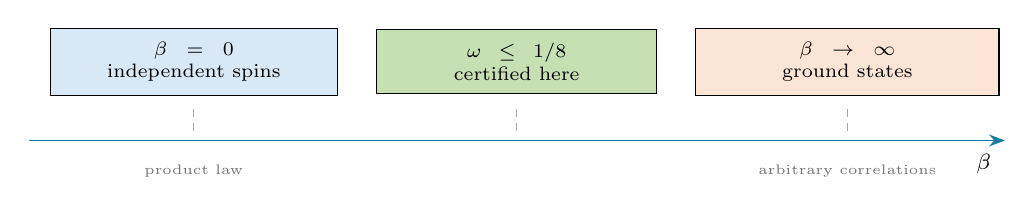
\begin{tikzpicture}[every node/.style={font=\scriptsize}]
\draw[arrow] (.2,0)--(12.6,0) node[below left=2pt] {\footnotesize$\beta$};
\node[box,fill=SoftBlue,text width=3.3cm] at (2.3,1.0) {$\beta=0$\\independent spins};
\node[box,fill=SoftGreen,text width=3.2cm] at (6.4,1.0) {$\omega\le 1/8$\\certified here};
\node[box,fill=SoftPeach,text width=3.5cm] at (10.6,1.0) {$\beta\to\infty$\\ground states};
\draw[black!35,densely dashed] (2.3,0.12)--(2.3,0.42);
\draw[black!35,densely dashed] (6.4,0.12)--(6.4,0.42);
\draw[black!35,densely dashed] (10.6,0.12)--(10.6,0.42);
\node[font=\tiny,black!55,anchor=north] at (2.3,-0.18) {product law};
\node[font=\tiny,black!55,anchor=north] at (10.6,-0.18) {arbitrary correlations};
\end{tikzpicture}
\end{center}
\uncover<2->{\textbf{Where Gibbs states appear.} Harrow--Wei's simulated annealing runs coherent Gibbs states to estimate partition functions; the classical outer loop proposes $x\sim\mu_\beta$.}
\uncover<3->{\takeaway{At low temperature a ferromagnet concentrates on aligned states: a global label can vary while every single-spin flip has vanishing influence.}}
\note{The obstruction is to a flip-influence theorem, not to mean simulation --- that distinction is the next slide.}
\end{frame}


% \begin{frame}{Which Gibbs models are worth chasing?}
% \band{Influence AA and query AA differ, and they come apart.}
% {\scriptsize
% \renewcommand{\arraystretch}{1.04}
% \begin{center}
% \begin{tabular}{@{}p{5.9cm}ccp{3.8cm}@{}}
% \hline
% \textbf{model \; (regime)} & \textbf{infl.} & \textbf{query} & \textbf{status}\\
% \hline
% product law, any alphabet \; (all $T$) & $\checkmark$ & $\checkmark$ & GMRR\\
% uniform slice, fixed weight \; (all $T$) & $\checkmark$ & $\checkmark$ & GMRR\\
% \hline
% Gibbs, $\omega\le 1/8$ \; (high $T$) & $?$ & $\checkmark$ & this work\\
% Ising on $\mathbb Z^d$, $\beta|J|\le 1/(16d)$ \; (high $T$) & $?$ & $\checkmark$ & Theorem 1.1\\
% 1D Ising chain \; (in between) & \textcolor{GuideBlue}{$\star\checkmark/\star\times$} & \textcolor{GuideBlue}{$\star\checkmark$} & decay; infl.\ high $T$\\
% \hline
% ferromagnet, ground states \; ($T=0$) & $\times$ & $\checkmark$ & MAJ$_3$ vs.\ 1 query\\
% \hline
% Curie--Weiss, $\beta>1$ \; (none known) & \textcolor{GuideBlue}{$\star\times$} & $?$ & aligned magnetization\\
% hard-core, high activity \; (none known) & \textcolor{GuideBlue}{$\star\times$} & $?$ & max.\ independent sets\\
% \hline
% \end{tabular}
% \end{center}}
% {\tiny\color{black!60} $\checkmark$ proved \;\textperiodcentered\; $\times$ counterexample \;\textperiodcentered\; $?$ open \;\textperiodcentered\; \textcolor{GuideBlue}{$\star$} our conjecture --- debt, not result\par}
% \takeaway{Influence is the fragile half: it dies at low temperature while mean simulation survives.}
% \credit{GMRR for the product and slice rows; Theorem 1.1 for rows 3--4.}
% \note{No Gibbs law is known to us where query AA fails. Row 5: the 1D chain has exponential decay at every beta, so the history argument should go through with larger L and B; influence, however, should fail once beta|J| is large, because MAJ_3 changes only near the O(e^{-2 beta J n}) interfaces. Row 7: above criticality the magnetization concentrates on two values, so a sign-of-magnetization function has variance but vanishing resampling influence. Row 8: at high activity the law sits on maximum independent sets, which are exactly a hard subset. Mark all three as conjectures if challenged; the two counterexample cells are what we would try to prove first.}
% \end{frame}

\begin{frame}{The model}
\band{$\displaystyle H(x)=-\sum_{|A|\ge2}J_A\chi_A(x)-\sum_i h_i x_i,\qquad \mu_\beta(x)=\frac{e^{-\beta H(x)}}{Z_\beta}$}
\begin{itemize}
\item $x\in\{\pm1\}^n$ is a configuration of $n$ spins, and $\chi_A(x)=\prod_{i\in A}x_i$.
\item Couplings $J_A$ and fields $h_i$ are arbitrary finite reals: any arity, any signs, any graph.
\item $\beta$ is the inverse temperature: larger $\beta$ means stronger correlations.
\end{itemize}
\takeaway{For which $\beta$ can a classical algorithm simulate quantum queries to $x\sim\mu_\beta$?}
\credit{Paper, \S1.}
\note{Only the model here. The answer depends on the Hamiltonian, which is the point of the next slide; our own regime comes after it.}
\end{frame}

\begin{frame}{Which Gibbs models are worth chasing?}
\band{A temperature threshold is one possible answer, not the only one.}
\begin{center}
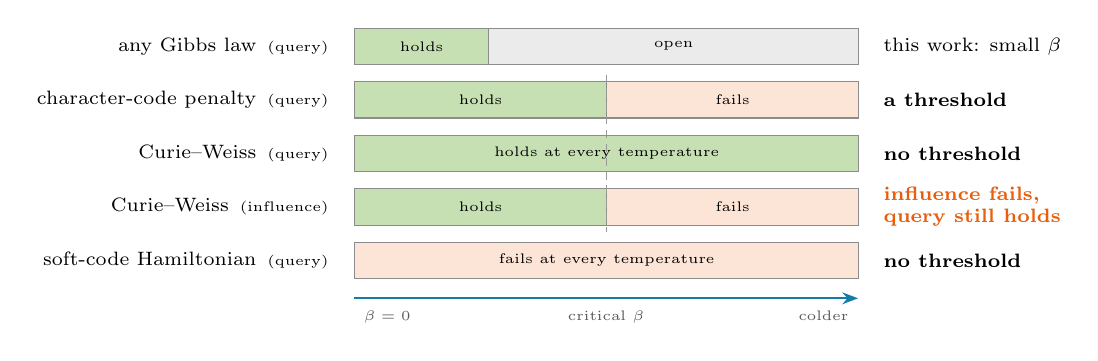
\begin{tikzpicture}[every node/.style={font=\scriptsize},
  seg/.style={draw=black!45,minimum height=4.6mm,inner sep=0pt,anchor=west,font=\tiny},
  ok/.style={seg,fill=SoftGreen}, no/.style={seg,fill=SoftPeach}, un/.style={seg,fill=black!8},
  lab/.style={anchor=east,align=right,font=\scriptsize},
  ver/.style={anchor=west,align=left,font=\scriptsize}]
% bars run from beta = 0 (left) to low temperature (right); total length 6.4cm
\node[lab] at (-.2,0) {any Gibbs law \,{\tiny(query)}};
\node[ok,minimum width=1.7cm] at (0,0) {holds};
\node[un,minimum width=4.7cm] at (1.7,0) {open};
\node[ver] at (6.6,0) {this work: small $\beta$};

\node[lab] at (-.2,-.68) {character-code penalty \,{\tiny(query)}};
\node[ok,minimum width=3.2cm] at (0,-.68) {holds};
\node[no,minimum width=3.2cm] at (3.2,-.68) {fails};
\node[ver] at (6.6,-.68) {\textbf{a threshold}};

\node[lab] at (-.2,-1.36) {Curie--Weiss \,{\tiny(query)}};
\node[ok,minimum width=6.4cm] at (0,-1.36) {holds at every temperature};
\node[ver] at (6.6,-1.36) {\textbf{no threshold}};

\node[lab] at (-.2,-2.04) {Curie--Weiss \,{\tiny(influence)}};
\node[ok,minimum width=3.2cm] at (0,-2.04) {holds};
\node[no,minimum width=3.2cm] at (3.2,-2.04) {fails};
\node[ver,text=NoteOrange] at (6.6,-2.04) {\textbf{influence fails,}\\\textbf{query still holds}};

\node[lab] at (-.2,-2.72) {soft-code Hamiltonian \,{\tiny(query)}};
\node[no,minimum width=6.4cm] at (0,-2.72) {fails at every temperature};
\node[ver] at (6.6,-2.72) {\textbf{no threshold}};

\draw[black!40,densely dashed] (3.2,-.36)--(3.2,-2.36);
\draw[arrow] (0,-3.2)--(6.4,-3.2);
\node[font=\tiny,black!65,anchor=north west] at (0,-3.24) {$\beta=0$};
\node[font=\tiny,black!65,anchor=north] at (3.2,-3.24) {critical $\beta$};
\node[font=\tiny,black!65,anchor=north east] at (6.4,-3.24) {colder};
\end{tikzpicture}
\end{center}
\vspace{-2mm}
\takeaway{Temperature regimes say more than influence: influence can fail where query simulation still holds.}
\credit{Team notes: threshold theory and Hamiltonian classification. All rows assume uniform-input AA.}
\note{Query means mean classical simulation of the acceptance probability; influence means the influential-coordinate inequality under the Gibbs law. Row 1 is Theorem 1.1; beyond the certified regime nothing general is known. Row 2: the character-code penalty family holds for fixed beta below its critical value and fails at and above it; the numerical value depends on the energy normalisation. Rows 3--4: Curie--Weiss is permutation-invariant, so query simulation holds at every temperature, while the influence inequality holds for beta at most 1 and fails above it, witnessed by the magnetisation. Row 5: the soft-code family fails at every fixed positive beta; its interaction order is unbounded. Each model has its own critical beta; the common dashed line is schematic. Backup: the set of good temperatures need not even be an interval; a three-level code construction holds exactly on [0,1) and (2,infinity].}
\end{frame}


\begin{frame}{The regime we certify}
\band{Query simulation holds whenever $\beta$ is small compared with the coupling at every spin.}
\begin{center}
{\colorbox{SoftGreen}{\parbox{0.88\textwidth}{\centering $\displaystyle \beta\;\le\;\frac{1}{8\,\max_i\sum_{A\ni i,\ |A|\ge2}(|A|-1)\,|J_A|}$}}}
\end{center}
\uncover<2->{\textbf{What the sum charges.} Each coupling at spin $i$, weighted by how many other spins it involves. For pairwise couplings it is just $\sum_j|J_{ij}|$.}

\uncover<3->{\textbf{What it does not see.} The fields $h_i$, the number of spins, the graph, and the signs of the couplings.}
\takeaway{A sufficient condition --- not a bare Dobrushin threshold, and not a claim to cover every unique law.}
\credit{Paper, \S1 and Theorem 1.1.}
\note{This is the first bar of the previous slide made precise. Arbitrary finite fields and pinnings are admitted; the constant is dimension-free; no conclusion follows from a uniqueness condition such as alpha < 1. The paper calls beta times this weighted sum omega and states the condition as omega at most 1/8.}
\end{frame}


\begin{frame}{Theorem 1.1: what the guarantee says}
\begin{columns}[T,onlytextwidth]
\column{.52\textwidth}
\centering
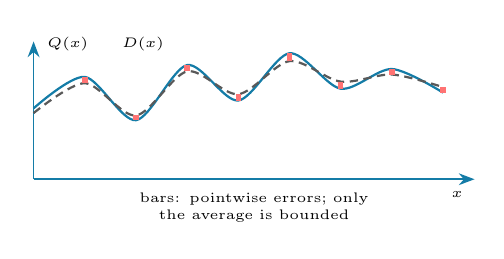
\begin{tikzpicture}[every node/.style={font=\tiny}]
\draw[arrow] (0,0)--(5.6,0) node[below left=1pt] {$x$};
\draw[arrow] (0,0)--(0,1.75);
\draw[GuideBlue,thick] plot[smooth] coordinates
 {(0,0.9) (0.65,1.3) (1.3,0.75) (1.95,1.45) (2.6,1.0) (3.25,1.6) (3.9,1.15) (4.55,1.4) (5.2,1.1)};
\draw[black!65,thick,densely dashed] plot[smooth] coordinates
 {(0,0.84) (0.65,1.22) (1.3,0.81) (1.95,1.37) (2.6,1.08) (3.25,1.5) (3.9,1.24) (4.55,1.33) (5.2,1.17)};
\foreach \x/\a/\b in {0.65/1.3/1.22,1.3/0.75/0.81,1.95/1.45/1.37,2.6/1.0/1.08,3.25/1.6/1.5,3.9/1.15/1.24,4.55/1.4/1.33,5.2/1.1/1.17}{
  \draw[red!55,line width=2pt] (\x,\a)--(\x,\b);}
\node[anchor=west] at (0.05,1.72) {$Q(x)$};
\node[anchor=west] at (1.0,1.72) {$D(x)$};
\node[anchor=north,text width=5.4cm,align=center] at (2.8,-0.05) {bars: pointwise errors; only the average is bounded};
\end{tikzpicture}
\column{.45\textwidth}
\centering\colorbox{SoftGreen}{\parbox{0.92\linewidth}{\centering\small\textbf{Theorem 1.1}\\[1pt] $\mathbb{E}_{\mu_\beta}|D-Q|\le e$\\[1pt] $M=O(T^{18}e^{-28})$}}
\end{columns}
\band{Mean, not pointwise. \; Queries, not runtime. \; The algorithm is data.}
\uncover<2->{\small Mean: no claim that $D(x)=Q(x)$ for each $x$. Queries: offline computation is free. Data: the construction uses the oracles and states of $\mathcal A_Q$, not just $Q(x)$.}
\takeaway{Everything that follows: how is $D$ built, and where does $T^{18}$ come from?}
\note{Do not open with full Dobrushin. State omega, mean error, free computation, the target. The three conventions return in the last slide.}
\end{frame}

\begin{frame}{The Gibbs update rule}
\band{Pick one spin. Forget its value. Redraw it, given the spins it interacts with.}
\begin{center}
\begin{tikzpicture}[every node/.style={font=\small},
  sp/.style={circle,draw=black!45,minimum size=6.5mm,inner sep=0pt},
  up/.style={sp,fill=SoftBlue}, dn/.style={sp,fill=SoftPeach}]
\foreach \sx in {0,5.2}{
  \begin{scope}[shift={(\sx,0)}]
    \node[up] (l) at (-1.15,0) {$+$};
    \node[dn] (r) at (1.15,0) {$-$};
    \node[up] (t) at (0,.95) {$+$};
    \node[up] (b) at (0,-.95) {$+$};
    \foreach \n in {l,r,t,b}{\draw[black!35] (0,0)--(\n);}
  \end{scope}}
\node[sp,fill=Highlight,draw=NoteOrange,thick] at (0,0) {?};
\node[up,draw=GuideBlue,thick] at (5.2,0) {$+$};
\draw[arrow,line width=1.1pt] (1.9,0)--node[above,font=\scriptsize]{redraw}(3.3,0);
\node[anchor=west,align=left,font=\small,text width=5.4cm] at (7.0,0)
  {The neighbours set the odds:\\[3pt]
   $\Pr[\,+\,]=\tfrac12\bigl(1+\tanh(\beta\cdot\text{pull})\bigr)$\\[3pt]
   {\scriptsize pull = what the neighbours and the field favour}};
\end{tikzpicture}
\end{center}
\begin{itemize}
\item<2-> \textbf{It keeps a Gibbs sample Gibbs.} Apply it to $x\sim\mu_\beta$ and the result is again a sample from $\mu_\beta$.
\item<3-> \textbf{High temperature means a weak pull.} The neighbours shift the odds only slightly, so most redraws could be made without looking at them.
\end{itemize}
\uncover<4->{\takeaway{Next: write each redraw as an independent random rule, which usually says ``ignore the neighbours''.}}
\credit{Known as heat-bath or Glauber dynamics, or the Gibbs sampler.}
\note{This is the only dynamics in the talk and it is a proof device: nobody runs it and no mixing time is claimed. The exact rule is $p_i(y\mid\eta)=(1+y\tanh(\beta h_i+u_i(\eta)))/2$, where $u_i$ is the local field from the couplings. Stationarity holds at every temperature. The high-temperature condition $\omega\le1/8$ is what makes the dependence on the neighbours weak, and the next slide turns that into random rules that are constants most of the time.}
\end{frame}

\begin{frame}{Move independence into the update history}
\band{We inject $X$ into a larger, independent space that we can deal with.}
\begin{center}
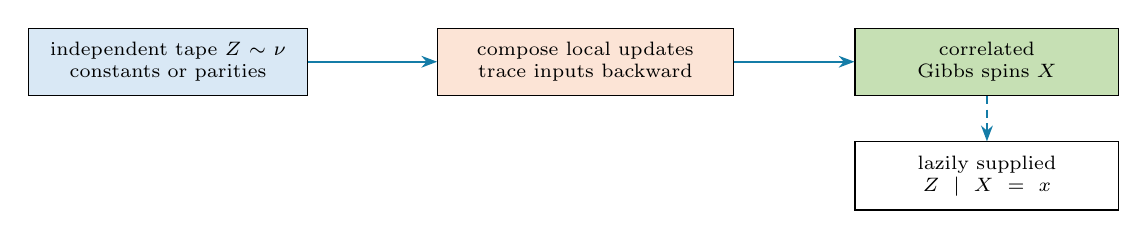
\begin{tikzpicture}[every node/.style={font=\scriptsize}]
\node[box,fill=SoftBlue,text width=3.2cm] (z) at (0,0) {independent tape $Z\sim\nu$\\constants or parities};
\node[box,fill=SoftPeach,text width=3.4cm] (h) at (5.3,0) {compose local updates\\trace inputs backward};
\node[box,fill=SoftGreen,text width=3.0cm] (x) at (10.4,0) {correlated\\Gibbs spins $X$};
\node[box,fill=white,text width=3.0cm] (c) at (10.4,-1.45) {lazily supplied\\ $Z\mid X=x$};
\draw[arrow] (z)--(h); \draw[arrow] (h)--(x);
\draw[arrow,densely dashed] (x)--(c);
\end{tikzpicture}
\end{center}
\uncover<2->{A constant update stops a dependency; a parity reads the spins it uses. Each event draws its own coin: \emph{the tape is a product law, its outputs are not.}}
\uncover<3->{\takeaway{Supports contract: expected reads per event are at most $\vartheta/2=\frac{80}{169}$.}}
\credit{Overview, \S4.2: the update-map lemma.}
\note{Say out loud that a constant map reading nothing makes whole branches free. Emphasise a private prior coin per event and independence across events before conditioning.}
\end{frame}

\begin{frame}{What a history looks like}
\band{$n$ spins, redrawn one at a time, for $L$ sweeps. One rule per redraw.}
\begin{center}
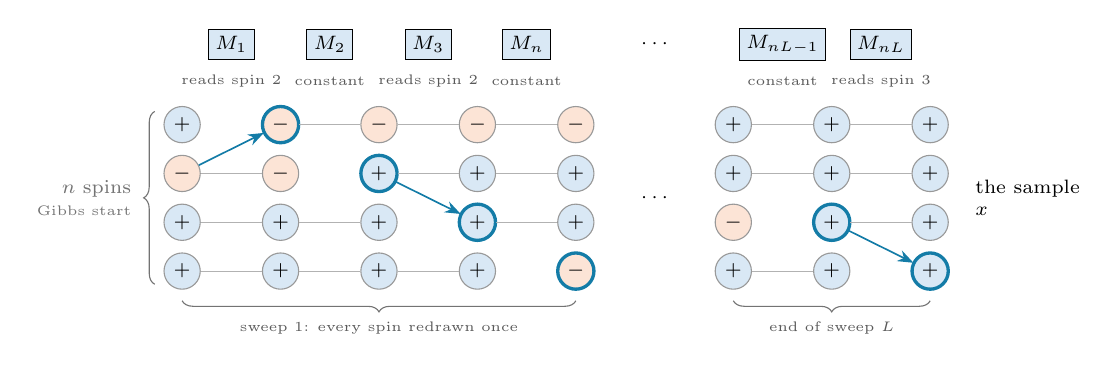
\begin{tikzpicture}[every node/.style={font=\scriptsize},
  sp/.style={circle,draw=black!40,minimum size=4.6mm,inner sep=0pt},
  cell/.style={sp,fill=#1}]
% columns are configurations (time runs left to right); rows are spins
\foreach \k/\x/\vals in {
  0/0/{+/SoftBlue,-/SoftPeach,+/SoftBlue,+/SoftBlue},
  1/1.25/{-/SoftPeach,-/SoftPeach,+/SoftBlue,+/SoftBlue},
  2/2.5/{-/SoftPeach,+/SoftBlue,+/SoftBlue,+/SoftBlue},
  3/3.75/{-/SoftPeach,+/SoftBlue,+/SoftBlue,+/SoftBlue},
  4/5.0/{-/SoftPeach,+/SoftBlue,+/SoftBlue,-/SoftPeach},
  5/7.0/{+/SoftBlue,+/SoftBlue,-/SoftPeach,+/SoftBlue},
  6/8.25/{+/SoftBlue,+/SoftBlue,+/SoftBlue,+/SoftBlue},
  7/9.5/{+/SoftBlue,+/SoftBlue,+/SoftBlue,+/SoftBlue}}{
  \foreach \v/\col [count=\r] in \vals {
    \node[cell=\col] (c\k-\r) at (\x,{-.62*(\r-1)}) {$\v$};}}
% each redraw: the other spins are carried over unchanged; one spin is rewritten
\foreach \k/\u/\lab/\d in {1/1/{M_1}/{reads spin 2},2/2/{M_2}/{constant},
    3/3/{M_3}/{reads spin 2},4/4/{M_n}/{constant},
    6/3/{M_{nL-1}}/{constant},7/4/{M_{nL}}/{reads spin 3}}{
  \pgfmathtruncatemacro\j{\k-1}
  \foreach \r in {1,...,4}{\ifnum\r=\u\else\draw[black!30] (c\j-\r)--(c\k-\r);\fi}
  \node[sp,draw=GuideBlue,very thick] at (c\k-\u) {};
  \node[box,fill=SoftBlue,inner sep=2.5pt] at ($(c\j-1)!.5!(c\k-1)+(0,1.02)$) {$\lab$};
  \node[font=\tiny,black!65] at ($(c\j-1)!.5!(c\k-1)+(0,.55)$) {\d};}
\draw[arrow] (c0-2)--(c1-1);
\draw[arrow] (c2-2)--(c3-3);
\draw[arrow] (c6-3)--(c7-4);
\node at (6.0,-.93) {$\cdots$};
\node at (6.0,1.02) {$\cdots$};
\draw[decorate,decoration={brace,amplitude=4pt},black!55]
  ($(c0-4.south west)+(-.18,0)$)--($(c0-1.north west)+(-.18,0)$)
  node[midway,left=5pt,align=right,font=\scriptsize]{$n$ spins\\{\tiny Gibbs start}};
\node[anchor=west,align=left,font=\scriptsize] at ($(c7-2)!.5!(c7-3)+(.45,0)$) {the sample\\$x$};
\draw[decorate,decoration={brace,mirror,amplitude=4pt},black!55]
  ($(c0-4.south)+(0,-.14)$)--($(c4-4.south)+(0,-.14)$)
  node[midway,below=4pt,font=\tiny,black!65]{sweep $1$: every spin redrawn once};
\draw[decorate,decoration={brace,mirror,amplitude=4pt},black!55]
  ($(c5-4.south)+(0,-.14)$)--($(c7-4.south)+(0,-.14)$)
  node[midway,below=4pt,font=\tiny,black!65]{end of sweep $L$};
\end{tikzpicture}
\end{center}
\vspace{-2mm}
{\small Blue ring: the spin being redrawn. Blue arrow: a spin its rule reads. Grey line: carried over unchanged.}
\uncover<2->{\takeaway{Arrows point one way, forward in time. A constant rule reads nothing. The rules $M_1,\dots,M_{nL}$ are the tape.}}
\note{Drawn with n = 4. Each column is a full configuration of the n spins; consecutive columns differ in at most one spin. A sweep is n redraws, so the history has nL redraws and nL + 1 configurations. The rule at each redraw is drawn independently in advance: here M_1 copies spin 2, M_2 is a constant, and so on. The last column is the Gibbs sample x that the simulator is actually given; everything to its left is the history attached to it.}
\end{frame}


\begin{frame}{The key lemma: the hidden randomness splits into simple pieces}
\band{Attach to a Gibbs sample $x$ a history that could have produced it, and the independent update rules that drove that history.}
\begin{center}
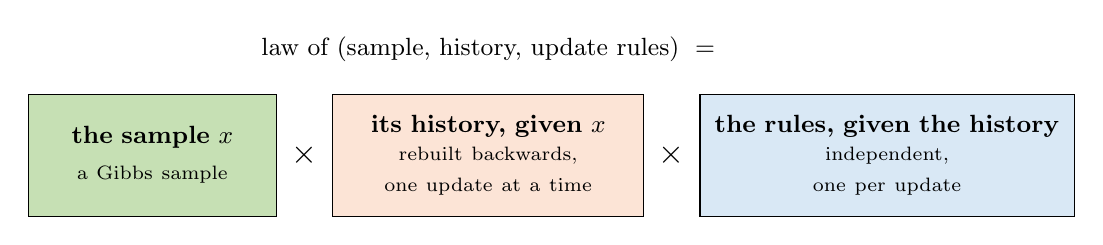
\begin{tikzpicture}[every node/.style={font=\small},node distance=7mm]
\node[box,fill=SoftGreen,text width=2.8cm,minimum height=1.55cm] (a)
  {\textbf{the sample $x$}\\[2pt]{\scriptsize a Gibbs sample}};
\node[box,fill=SoftPeach,text width=3.6cm,minimum height=1.55cm,right=of a,visible on=<2->] (b)
  {\textbf{its history, given $x$}\\[2pt]{\scriptsize rebuilt backwards,\\one update at a time}};
\node[box,fill=SoftBlue,text width=4.4cm,minimum height=1.55cm,right=of b,visible on=<3->] (c)
  {\textbf{the rules, given the history}\\[2pt]{\scriptsize independent,\\one per update}};
\node[font=\large,visible on=<2->] at ($(a.east)!.5!(b.west)$) {$\times$};
\node[font=\large,visible on=<3->] at ($(b.east)!.5!(c.west)$) {$\times$};
\node[anchor=south,font=\small] at ($(b.north)+(0,.28)$)
  {law of (sample, history, update rules) \;=};
\end{tikzpicture}
\end{center}
\uncover<4->{\begin{center}\small Every piece is local: it involves one spin and the few spins next to it.\end{center}}
\uncover<5->{\takeaway{So from $x$ alone, the independent randomness behind it can be generated piece by piece, on demand.}}
\credit{Paper, Lemma 3.2.}
\note{This is the lemma in the form the proof uses. The update rules are the tape: one random rule per update, independent of each other, chosen so that applying them to a Gibbs sample gives a Gibbs sample. The joint law of everything can then be written starting from the end: first the sample, then the earlier history given the sample, then the rules given the whole history. The second factor is a chain of single-spin resamplings in reverse order. The third is a product over updates, because the history imposes one constraint per rule. Caveat if asked: the rules are independent given the whole history, not given $x$ alone, which is why the history is rebuilt first. Nobody claims $x$ was produced by such a history; the history is attached to it.}
\end{frame}



\begin{frame}{The estimator $D$: offline and online}
\begin{center}
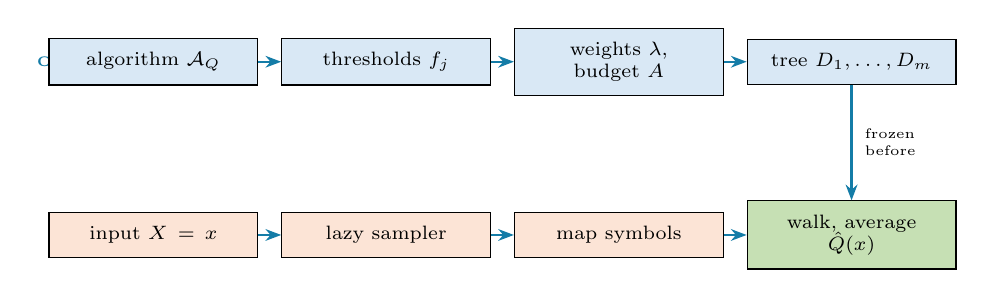
\begin{tikzpicture}[every node/.style={font=\scriptsize},node distance=2.9mm]
\node[font=\tiny\bfseries,GuideBlue,anchor=east] at (-0.2,1.2) {OFFLINE};
\node[font=\tiny\bfseries,black!60,anchor=east] at (-0.2,-1.0) {ONLINE};
\node[box,fill=SoftBlue,text width=2.3cm] (a1) at (0,1.2) {algorithm $\mathcal A_Q$};
\node[box,fill=SoftBlue,text width=2.3cm,right=of a1] (a2) {thresholds $f_j$};
\node[box,fill=SoftBlue,text width=2.3cm,right=of a2] (a3) {weights $\lambda$, budget $A$};
\node[box,fill=SoftBlue,text width=2.3cm,right=of a3] (a4) {tree $D_1,\dots,D_m$};
\draw[arrow] (a1)--(a2); \draw[arrow] (a2)--(a3); \draw[arrow] (a3)--(a4);
\node[box,fill=SoftPeach,text width=2.3cm] (b1) at (0,-1.0) {input $X=x$};
\node[box,fill=SoftPeach,text width=2.3cm,right=of b1] (b2) {lazy sampler};
\node[box,fill=SoftPeach,text width=2.3cm,right=of b2] (b3) {map symbols};
\node[box,fill=SoftGreen,text width=2.3cm,right=of b3] (b4) {walk, average\\ $\hat Q(x)$};
\draw[arrow] (b1)--(b2); \draw[arrow] (b2)--(b3); \draw[arrow] (b3)--(b4);
\draw[arrow,line width=0.9pt] (a4.south)--(b4.north) node[midway,right=1pt,font=\tiny,align=left] {frozen\\ before};
\end{tikzpicture}
\end{center}
{\small\textbf{Only the second row touches the physical input.}}
\begin{itemize}
\item \textbf{Offline}, free: history $\to$ weights $\to$ tree, frozen.
\item \textbf{Online}, charged: the lazy sampler answers exactly the symbols asked for.
\end{itemize}
\takeaway{The rest of this part fills in these boxes; the next part pays the three debts the picture takes out.}
\note{Keep pointing back to this picture: every later frame is either a box being filled in or a debt being paid.}
\end{frame}


\begin{frame}{Offline: certificates on a product of symbol alphabets}
\band{A coordinate holds a whole update map, and its marginal may be biased.}
\begin{center}
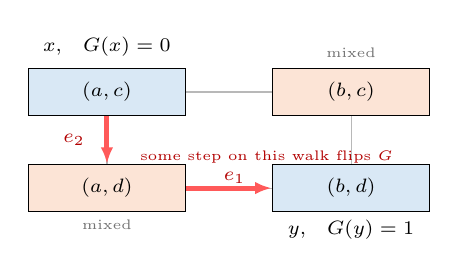
\begin{tikzpicture}[every node/.style={font=\scriptsize}]
% corner grid
\node[box,fill=SoftBlue,minimum width=2.0cm,minimum height=0.56cm] (xc) at (0,1.22) {$(a,c)$};
\node[box,fill=SoftPeach,minimum width=2.0cm,minimum height=0.56cm] (bc) at (3.1,1.22) {$(b,c)$};
\node[box,fill=SoftPeach,minimum width=2.0cm,minimum height=0.56cm] (ad) at (0,0) {$(a,d)$};
\node[box,fill=SoftBlue,minimum width=2.0cm,minimum height=0.56cm] (bd) at (3.1,0) {$(b,d)$};
\draw[black!28] (xc)--(bc); \draw[black!28] (xc)--(ad);
\draw[black!28] (bc)--(bd); \draw[black!28] (ad)--(bd);
% the one-coordinate walk
\draw[red!65,line width=1.8pt,-{Latex[length=2.1mm]}]
  (xc.south)--(ad.north);
\draw[red!65,line width=1.8pt,-{Latex[length=2.1mm]}]
  (ad.east)--(bd.west);
\node[font=\tiny,text=red!70!black,anchor=west] at (0.30,0.40) {some step on this walk flips $G$};
% tags
\node[font=\scriptsize,anchor=south] at (0,1.55) {$x$, \; $G(x)=0$};
\node[font=\tiny,black!55,anchor=south] at (3.1,1.53) {mixed};
\node[font=\scriptsize,anchor=north] at (3.1,-0.28) {$y$, \; $G(y)=1$};
\node[font=\tiny,black!55,anchor=north] at (0,-0.28) {mixed};
% coordinate ticks on the walk
\node[font=\scriptsize,text=red!70!black,anchor=east] at (-0.16,0.61) {$e_2$};
\node[font=\scriptsize,text=red!70!black,anchor=south] at (1.62,-0.06) {$e_1$};
\end{tikzpicture}
\end{center}
\vspace{-3mm}
{\small Weight each corner by the product of its two marginals --- independence makes that the joint probability --- then sum the boundary inequality over boxes.}
\takeaway{Were every coordinate weakly influential, $x$ could be edited into $y$ below budget. So cheap evidence forces some unread $i$ with $I_i\ge m(C)^2/(32A^2)$.}
\credit{Paper, Lemmas 3.5--3.6; box input from Huffstutler et al., Lemma 4.}
\note{Read it as the contrapositive, which is how the tree uses it: a cheap certificate plus two classes of positive mass forces influence somewhere. The walk from x to y is what converts a statement about a pair of tapes into a statement about one coordinate. Independence enters exactly once, in the weight of a corner.}
\end{frame}


\begin{frame}{Offline: from query attention to a certificate}
{\small Where the weights come from: how often the source algorithm \emph{looks} at each map event.}
\begin{columns}[T,onlytextwidth]
\column{.49\textwidth}
\centering
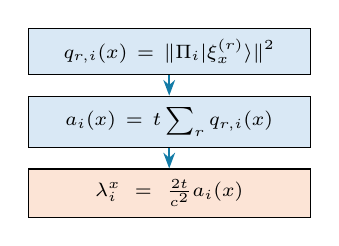
\begin{tikzpicture}[every node/.style={font=\scriptsize},node distance=2.6mm]
\node[box,fill=SoftBlue,text width=3.3cm,inner sep=4pt] (a) {$q_{r,i}(x)=\|\Pi_i|\xi_x^{(r)}\rangle\|^2$};
\node[box,fill=SoftBlue,text width=3.3cm,inner sep=4pt,below=of a] (b) {$a_i(x)=t\sum_r q_{r,i}(x)$};
\node[box,fill=SoftPeach,text width=3.3cm,inner sep=4pt,below=of b] (c) {$\lambda_i^x=\frac{2t}{c^2}a_i(x)$};
\draw[arrow] (a)--(b); \draw[arrow] (b)--(c);
\end{tikzpicture}
\column{.49\textwidth}
\centering
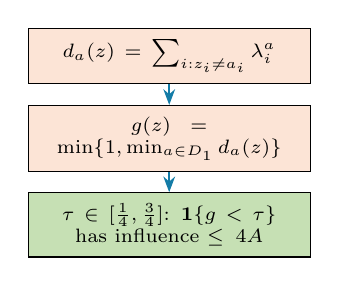
\begin{tikzpicture}[every node/.style={font=\scriptsize},node distance=2.6mm]
\node[box,fill=SoftPeach,text width=3.3cm,inner sep=4pt] (d) {$d_a(z)=\sum_{i:z_i\ne a_i}\lambda_i^a$};
\node[box,fill=SoftPeach,text width=3.3cm,inner sep=4pt,below=of d] (e) {$g(z)=\min\{1,\min_{a\in D_1}d_a(z)\}$};
\node[box,fill=SoftGreen,text width=3.3cm,inner sep=4pt,below=of e] (f) {$\tau\in[\frac14,\frac34]$: $\mathbf 1\{g<\tau\}$ has influence $\le 4A$};
\draw[arrow] (d)--(e); \draw[arrow] (e)--(f);
\end{tikzpicture}
\end{columns}
\band{$\displaystyle\sum_{i\in\Delta(x,y)}\min(\lambda_i^x,\lambda_i^y)\ge 1$, \qquad $\displaystyle\sum_i\lambda_i^x\le A=\frac{2t^2}{c^2}$.}
\uncover<2->{\takeaway{Weights give a Boolean function of bounded influence; averaging gives a good threshold.}}
\credit{Paper, \S9.1--9.2.}
\note{Why adversary data is indispensable: if the algorithm never looked at the coordinates where two tapes differ, the states would be nearly identical and it could not answer differently.}
\end{frame}


\begin{frame}{Offline: from threshold classifiers to mean error}
\begin{columns}[T,onlytextwidth]
\column{.49\textwidth}
\centering\colorbox{SoftBlue}{\strut Lemma 3.7}\par\medskip
{\footnotesize Query an influential symbol at each node. The minority mass $m(C)=\min\{\delta_0,\delta_1\}$ obeys
\[
\max_i I_i^{\mu\mid C}(G)\ \ge\ \frac{m(C)^2}{32A^2},
\]
and $\lceil 128A^3/\eta^2\rceil$ queries leave error mass at most $\eta$.}
\column{.49\textwidth}
\centering\colorbox{SoftPeach}{\strut Lemma 3.8}\par\medskip
{\footnotesize Thresholds $j/m$ with margin $a$: say 0 clearly below, 1 clearly above, undefined between. Average the bits,
\[
D(z)=\frac1m\sum_{j} D_j(z),
\]
so $\mathbb E_\nu|D-Q\circ F_{L,B}|\le e/3$ by layer cake.}
\end{columns}
\band{Depth: $m\asymp a\asymp\eta\asymp e$, $A\asymp B^2T^2e^{-4}$, so $s=O((BT)^6e^{-15})=O(T^{18}e^{-27})$.}
\uncover<2->{\takeaway{A grid turns bits into a real value; the error is the mass of mistakes, not the error on one path.}}
\credit{Paper, Lemmas 3.7--3.8.}
\note{Unconditional error mass = probability of being both on-promise and wrong under the full product law. Thresholds near the true value may be off-promise, but only a small fraction of the grid lies there.}
\end{frame}


\begin{frame}{Online: lazy supply, one node at a time}
\band{The tree asks for map symbols; the sampler answers exactly those.}
\begin{columns}[T,onlytextwidth]
\column{.45\textwidth}
\centering
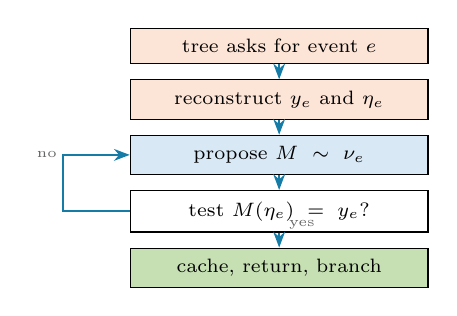
\begin{tikzpicture}[every node/.style={font=\scriptsize},node distance=1.9mm]
\node[box,fill=SoftPeach,text width=3.5cm,inner sep=4pt] (a) {tree asks for event $e$};
\node[box,fill=SoftPeach,text width=3.5cm,inner sep=4pt,below=of a] (b) {reconstruct $y_e$ and $\eta_e$};
\node[box,fill=SoftBlue,text width=3.5cm,inner sep=4pt,below=of b] (c) {propose $M\sim\nu_e$};
\node[box,fill=white,text width=3.5cm,inner sep=4pt,below=of c] (d) {test $M(\eta_e)=y_e$?};
\node[box,fill=SoftGreen,text width=3.5cm,inner sep=4pt,below=of d] (e) {cache, return, branch};
\draw[arrow] (a)--(b); \draw[arrow] (b)--(c); \draw[arrow] (c)--(d);
\draw[arrow] (d)--node[pos=0.42,anchor=south west,font=\tiny,black!60]{yes}(e);
\draw[arrow] (d.west)--++(-0.85,0)|-(c.west)
  node[pos=0.55,anchor=east,xshift=-1pt,font=\tiny,black!60]{no};
\end{tikzpicture}
\column{.52\textwidth}
{\small\textbf{$V(j,t)$} returns the value at site $j$ before event $t$: take the first update $u>t$ at $j$ (none: return $x_j$); otherwise alias to that node: cache hit returns, else expose the reverse map and recurse on its support.\\[1pt]
\textbf{Exact:} the first $M$ with $M(\eta_e)=y_e$ is Bayes on the recovered history.}
\end{columns}
\uncover<2->{\takeaway{Rejected proposals cost no support, so work follows the tree: expected $\frac{418}{89}s$ at source depth $s$.}}
\credit{Paper, Lemma 3.9 and \S12.}
\note{Walk one event out loud: reject the constant at empty support, accept the parity, then go back for the preceding event. Expected work counts history and source accesses; it is not a worst-case runtime.}
\end{frame}


\begin{frame}{Why $L$ sweeps and $B$ reads}
\band{Truncation creates two errors of different kinds.}
\begin{columns}[T,onlytextwidth]
\column{.46\textwidth}
\centering
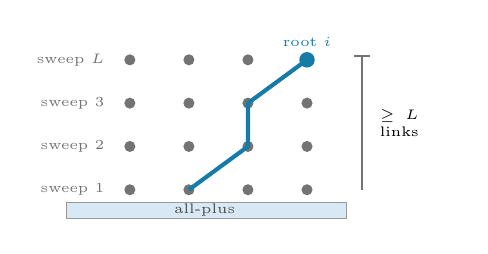
\begin{tikzpicture}[every node/.style={font=\scriptsize}]
\foreach \r/\yy/\lab in {0/0/{sweep $1$},1/0.55/{sweep $2$},2/1.10/{sweep $3$},3/1.65/{sweep $L$}}{
  \foreach \c in {1,...,4}{\fill[black!55] (\c*0.75,\yy) circle (2pt);}
  \node[font=\tiny,black!55,anchor=east] at (0.55,\yy) {\lab};}
\draw[GuideBlue,line width=1.5pt] (3.0,1.65)--(2.25,1.10)--(2.25,0.55)--(1.5,0);
\fill[GuideBlue] (3.0,1.65) circle (2.8pt);
\node[font=\tiny,GuideBlue,anchor=south] at (3.0,1.7) {root $i$};
\fill[SoftBlue] (-0.05,-0.36) rectangle (3.5,-0.16);
\draw[black!40] (-0.05,-0.36) rectangle (3.5,-0.16);
\node[font=\tiny,black!70] at (1.7,-0.26) {all-plus};
\draw[black!55,thick] (3.7,1.7)--(3.7,0);
\draw[black!55,thick] (3.6,1.7)--(3.8,1.7);
\node[font=\tiny,anchor=west,text width=0.9cm] at (3.8,0.85) {$\ge L$ links};
\end{tikzpicture}
\column{.5\textwidth}
{\small
\textbf{History depth $L$:} too few sweeps give error $\vartheta^{L}$, geometric.\\[2pt]
\textbf{Read cap $B$:} exceeding it costs $[B(1-\vartheta)]^{-1}$ by Markov.\\[2pt]
Neither bounds how long the true history was.}
\end{columns}
\band{$\displaystyle \Pr\bigl[F_{L,B}(Z)_i\ne x_i\mid X=x\bigr]\le \vartheta^{L}+[B(1-\vartheta)]^{-1}\le 2\delta=\gamma$}
\uncover<2->{\takeaway{$\delta=\frac{e^2}{288T^2}$, $L=\lceil\log(1/\delta)/\log(1/\vartheta)\rceil$, $B=\lceil 5408T^2/e^2\rceil$: every root is right except with probability $\gamma$.}}
\credit{Overview, \S7: truncation and the hybrid bound.}
\note{Keep the two errors apart: history truncation is geometric, read truncation is a Markov tail. B caps evaluation reads; it is not a claim about the physical history.}
\end{frame}


\begin{frame}{The three costs, and the cap}
\band{Spend one third of the allowed mean error on each step.}
\begin{center}
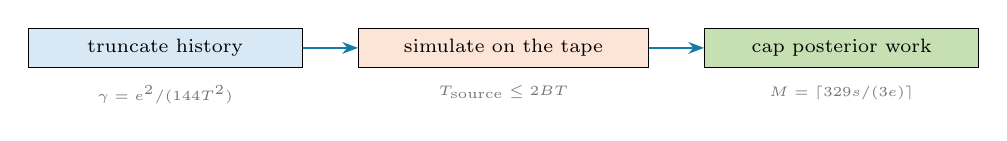
\begin{tikzpicture}[node distance=7mm,every node/.style={font=\scriptsize}]
\node[box,fill=SoftBlue,text width=3.2cm,inner sep=4pt] (a) {truncate history};
\node[box,fill=SoftPeach,text width=3.4cm,inner sep=4pt,right=of a] (b) {simulate on the tape};
\node[box,fill=SoftGreen,text width=3.2cm,inner sep=4pt,right=of b] (c) {cap posterior work};
\draw[arrow] (a)--(b); \draw[arrow] (b)--(c);
\node[font=\tiny,black!55,below=1mm of a] {$\gamma=e^2/(144T^2)$};
\node[font=\tiny,black!55,below=1mm of b] {$T_{\rm source}\le 2BT$};
\node[font=\tiny,black!55,below=1mm of c] {$M=\lceil 329s/(3e)\rceil$};
\end{tikzpicture}
\end{center}
{\small A root disagrees with probability at most $\gamma$, so the coherent evaluate--call--uncompute step costs
\[
4T\sqrt{\gamma}=4T\sqrt{\frac{e^2}{144T^2}}=\frac e3 .
\]}
\uncover<2->{\takeaway{source $e/3$ + hybrid $e/3$ + abort $e/3$ = $e$, with $M=O(T^{18}e^{-28})$.}}
\credit{Paper, Lemma 3.9 and Theorem 3.10.}
\note{The hybrid bound handles quantum queries in superposition, so a classical pathwise bound is not enough. One cap serves all classifiers; per-classifier caps would multiply the depth.}
\end{frame}


% \begin{frame}{What the theorem does not claim}
% {\small
% \begin{columns}[T,onlytextwidth]
% \column{.49\textwidth}
% \begin{itemize}
% \item \textbf{Not full Dobrushin.} $\omega\le 1/8$ is the condition; a uniqueness threshold gives nothing.
% \item \textbf{Not polynomial-influence AA.} No bound on $\mathrm{Inf}_i(p)$ under $\mu_\beta$.
% \item \textbf{Not efficient sampling.} No sampler, no mixing time.
% \item \textbf{Not pointwise.} Only $\mathbb E|D-Q|\le e$.
% \end{itemize}
% \column{.49\textwidth}
% \begin{itemize}
% \item \textbf{Not runtime-efficient.} Offline work is unbounded; a bad proposal tape escapes the cap.
% \item \textbf{Not product posteriors.} Independence needs a complete trajectory.
% \item \textbf{Not branchwise monotone.} Expectations, not paths.
% \item \textbf{Not formalised.} Imported box inequalities are external theorems.
% \end{itemize}
% \end{columns}}
% \takeaway{Narrow and exact: deterministic, polynomially many spin queries, mean error $e$, at certified high temperature.}
% \credit{Paper, \S17.}
% \note{Do not rush this slide: most hostile questions are answered here before they are asked. The two nobody expects are branchwise monotonicity and the absence of a proposal-length bound.}
% \end{frame}

% Ians stuff%

% ============================================================
% HARD SECTORS 1. WHERE AA FAILS, AND WHY
% ============================================================
\begin{frame}{Where AA fails for Gibbs laws}
\begin{center}
\footnotesize
\renewcommand{\arraystretch}{1.15}
\begin{tabular}{ll}
\textbf{Hamiltonian (repo)} & \textbf{AA fails at fixed}\\
\hline
Character-code Hamiltonian & $\beta\ge1$\\
Nonmonotone code energy & $1\le\beta\le2$ only\\
Soft-code Hamiltonian & every $\beta>0$\\
Dense three-local interactions & $\beta J>16\log2$\\
Bounded-degree pairwise Ising (with auxiliary spins) & $\beta j\ge1$
\end{tabular}
\end{center}

\uncover<2->{\band{Each proof finds inputs where the answer varies, but shallow
classical queries learn nothing about it. That alone rules out AA.}}

\uncover<3->{\small A \textbf{hard sector} for an accept/reject probability $p(x)$
is a set of inputs $H$ with:
\begin{center}
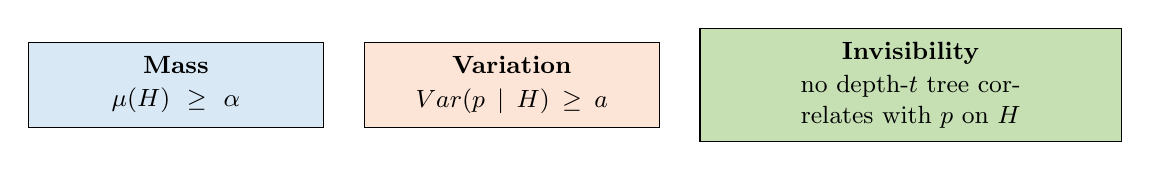
\begin{tikzpicture}[node distance=5mm]
\node[box,fill=SoftBlue,text width=3.4cm,font=\small] (c1)
  {\textbf{Mass}\\[1pt]$\mu(H)\ge\alpha$};
\node[box,fill=SoftPeach,text width=3.4cm,font=\small,right=of c1] (c2)
  {\textbf{Variation}\\[1pt]$\Var(p\mid H)\ge a$};
\node[box,fill=SoftGreen,text width=5.0cm,font=\small,right=of c2] (c3)
  {\textbf{Invisibility}\\[1pt]no depth-$t$ tree correlates with $p$ on $H$};
\end{tikzpicture}
\end{center}}

\uncover<4->{\small\textbf{Example.} $p(x)=1$ exactly when $x_1x_2\cdots x_n=1$.
On uniform inputs, all inputs form a hard sector: $p$ is a fair coin, and no tree
with fewer than $n$ queries sees it.}

\note{In every row, one quantum query needs Omega(log n) classical queries at
constant error. Temperature ranges are from the repo: character code, weight
criterion; nonmonotone, exact set; soft code, all fixed beta; dense three-local,
beta J > 16 log 2; pairwise Ising, K(beta j) > log 2/32, for which beta j >= 1
suffices. Invisibility means |Cov(p,D | H)| <= gamma for every depth-t tree D.
A hard sector forces every depth-t tree to err by at least alpha(a - 2 gamma).
This rules out AA once t is far beyond poly(Q). The parity example only illustrates
the definition: quantum also needs n/2 queries for parity, so it is not a
counterexample to AA.}
\end{frame}


% ============================================================
% HARD SECTORS 2. THE CONVERSE
% ============================================================
\begin{frame}{The converse: the best classical guess builds a hard sector}
\begin{center}
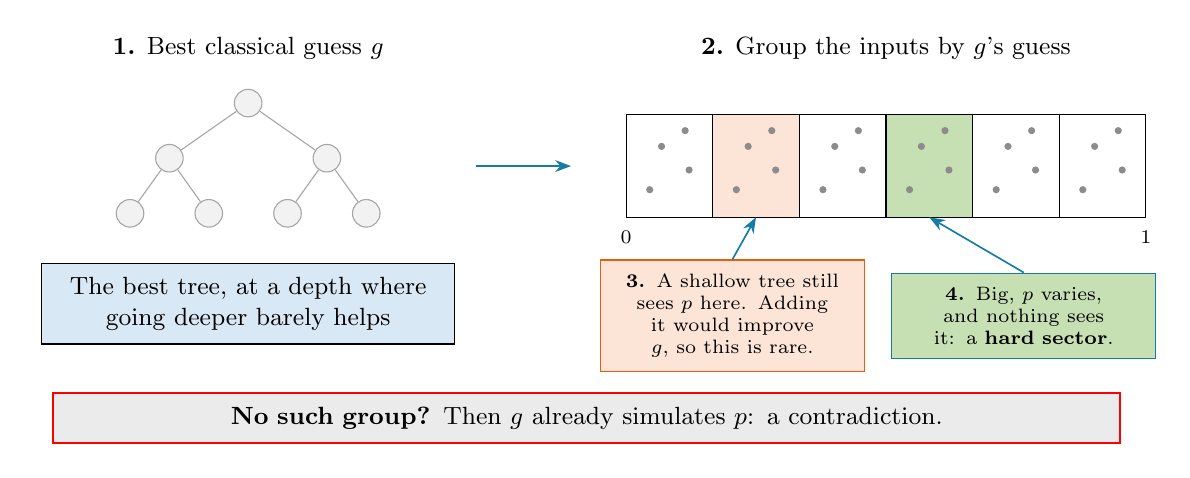
\begin{tikzpicture}[
 dn/.style={circle,draw=black!35,fill=black!5,minimum size=3.5mm,inner sep=0pt}
]
% 1: The best classical guess.
\node[font=\small] at (2.8,4.75) {\textbf{1.} Best classical guess $g$};
\node[dn] (r) at (2.8,4.05) {};
\node[dn] (a) at (1.8,3.35) {};
\node[dn] (b) at (3.8,3.35) {};
\foreach \n/\x in {l1/1.3,l2/2.3,l3/3.3,l4/4.3}{\node[dn] (\n) at (\x,2.65) {};}
\foreach \u/\v in {r/a,r/b,a/l1,a/l2,b/l3,b/l4}{\draw[black!35] (\u)--(\v);}
\node[box,fill=SoftBlue,text width=4.9cm,font=\small] at (2.8,1.5)
  {The best tree, at a depth where\\going deeper barely helps};

% 2: Group the inputs by the guess.
\draw[arrow,visible on=<2->] (5.7,3.25)--(6.9,3.25);
\node[font=\small,visible on=<2->] at (10.9,4.75)
  {\textbf{2.} Group the inputs by $g$'s guess};
% Fills first, so outlines and dots sit on top.
\fill[SoftPeach,visible on=<3->] (8.7,2.6) rectangle (9.8,3.9);
\fill[SoftGreen,visible on=<4->] (10.9,2.6) rectangle (12.0,3.9);
\begin{scope}[visible on=<2->]
  \foreach \i in {0,...,5}{
    \draw (7.6+1.1*\i,2.6) rectangle ++(1.1,1.3);
    \foreach \dx/\dy in {.3/.35,.8/.6,.45/.9,.75/1.1}{
      \fill[black!45] (7.6+1.1*\i+\dx,2.6+\dy) circle (1.3pt);}
  }
  \node[font=\scriptsize] at (7.6,2.35) {$0$};
  \node[font=\scriptsize] at (14.2,2.35) {$1$};
\end{scope}

% 3: Groups where a shallow tree still helps are rare.
\begin{scope}[visible on=<3->]
  \node[callout,text width=3.0cm,font=\scriptsize] (bad) at (8.95,1.35)
    {\textbf{3.} A shallow tree still sees $p$ here. Adding it would improve $g$,
     so this is rare.};
  \draw[arrow] (bad.north)--(9.25,2.6);
\end{scope}

% 4: The hard sector.
\begin{scope}[visible on=<4->]
  \node[box,fill=SoftGreen,draw=GuideBlue,text width=3.0cm,font=\scriptsize]
    (hard) at (12.65,1.35)
    {\textbf{4.} Big, $p$ varies, and nothing sees it: a \textbf{hard sector}.};
  \draw[arrow] (hard.north)--(11.45,2.6);
\end{scope}

% 5: Otherwise the guess already simulates p.
\node[conclusion,text width=13.2cm,font=\small,visible on=<5->] at (7.1,.05)
  {\textbf{No such group?} Then $g$ already simulates $p$: a contradiction.};

\path (0,-.35) rectangle (14.4,5.0);
\end{tikzpicture}
\end{center}

\uncover<6->{\takeaway{\footnotesize
\textbf{Theorem.} For every family of input laws $\mu_n$: AA fails \textbf{if and only if}
for every polynomial budget $P$ there are $n$, $Q$, $\varepsilon<1/8$, a $Q$-query $p$
and a set $H$ with
\[
\mu_n(H)\ge\frac{\varepsilon^3}{64},\qquad
\Var(p\mid H)\ge\frac{\varepsilon^2}{4},\qquad
|\operatorname{Cov}(p,D\mid H)|\le\frac{\varepsilon^2}{32}
\ \text{ for every tree $D$ of depth } t>P(Q,1/\varepsilon).
\]
\textbf{Cost.} If every tree of depth $\lceil512\,\varepsilon^{-5}\rceil\,t$ has mean
error $>\varepsilon$, such an $H$ exists at depth $t$, and a classical tree of that
depth decides membership in $H$.}}

\note{Step 1: the error of the best depth-jt tree starts at most 1/4 and only falls,
so some depth barely improves; take the best tree there. Step 2: within a group,
g is essentially constant. Step 3: so a tree that correlates with p in a group also
correlates with the error p - g, and appending it would lower the error; since depth
stopped helping, such groups have small total mass. Step 4: a large group with p
varying and no correlating tree is exactly a hard sector. If there is none, g has
error at most epsilon. Nothing quantum is used. AA means: one fixed polynomial P such
that every Q-query p has mean error at most epsilon against some tree of depth
P(Q,1/epsilon). The gamma here is for trees with outputs in [0,1]; with outputs in
[-1,1] it doubles to eps^2/16, as in the repo.}
\end{frame}


% ============================================================
% HARD SECTORS 3. HARD SECTORS AND ALGORITHMS
% ============================================================
\begin{frame}{Hard sectors as fingerprints of quantum algorithms}
\band{Simon: $f(x)=f(x\oplus s)$ for a hidden mask $s$. Quantum finds $s$ with
$O(m)$ queries; classical needs about $2^{m/2}$.}
\begin{center}
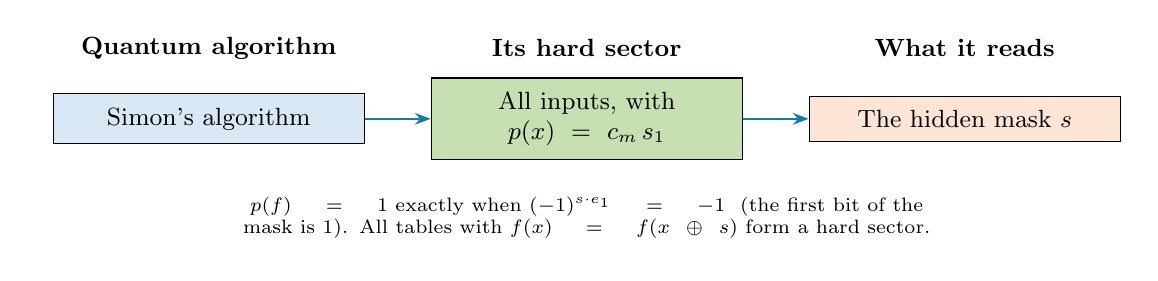
\begin{tikzpicture}
\node[font=\small\bfseries] at (2.3,2.75) {Quantum algorithm};
\node[font=\small\bfseries] at (7.1,2.75) {Its hard sector};
\node[font=\small\bfseries] at (11.9,2.75) {What it reads};
\node[box,fill=SoftBlue,text width=3.6cm,font=\small] (q) at (2.3,1.85)
  {Simon's algorithm};
\node[box,fill=SoftGreen,text width=3.6cm,font=\small] (h) at (7.1,1.85)
  {All inputs, with\\$p(x)=c_m\,s_1$};
\node[box,fill=SoftPeach,text width=3.6cm,font=\small] (o) at (11.9,1.85)
  {The hidden mask $s$};
\draw[arrow] (q)--(h);
\draw[arrow] (h)--(o);

\node[font=\scriptsize,text width=13.5cm,align=center,visible on=<2->] at (7.1,.6)
  {$p(f)=1$ exactly when $(-1)^{s\cdot e_1}=-1$ \ (the first bit of the mask is $1$).
   All tables with $f(x)=f(x\oplus s)$ form a hard sector.};

\path (0,.15) rectangle (14,3.0);
\end{tikzpicture}
\end{center}

\uncover<3->{\small\textbf{Theorem (robustness).} If a quantity is hidden from shallow
classical trees and a quantum algorithm computes it, even approximately, that algorithm
has a hard sector.}

\uncover<4->{\takeaway{Every quantum advantage leaves a hard sector. Can we
characterize quantum algorithms, or find new ones, through their hard sectors?}}
\end{frame}



% SLIDE 1% ============================================================
% 1. YZ RESULT
% ============================================================
\begin{frame}{[YZ22]: quantum advantage implies certified randomness}

\usebeamercolor{structure}
\colorlet{SlideAccent}{structure.fg}
\usebeamercolor{normal text}
\colorlet{SlideInk}{normal text.fg}

\begin{columns}[c,onlytextwidth]
\begin{column}{0.43\textwidth}
\centering
\begin{tikzpicture}[x=1cm,y=1cm,font=\scriptsize,
                   text=SlideInk]
  \draw[->,thick,SlideAccent] (0,0) -- (0,4.25)
    node[above,align=center]
    {Oracle queries\\(schematic, log scale)};

  \draw[SlideAccent,dashed,thick]
    (-.12,3.55) -- (3.6,3.55);
  \node[anchor=south west,align=left]
    at (.18,3.62)
    {$T$: classical lower bound\\for witness search};

  \begin{scope}[visible on=<2->]
    \draw[SlideAccent,thick] (-.12,.6) -- (.25,.6);
    \fill[SlideAccent] (0,.6) circle (2pt);
    \node[anchor=west,align=left,fill=SoftGreen,
          rounded corners=2pt,inner sep=5pt]
      at (.35,.6)
      {$Q$: quantum upper bound\\for witness search};
  \end{scope}
\end{tikzpicture}
\end{column}

\begin{column}{0.12\textwidth}
\centering
\uncover<3->{%
  {\usebeamercolor[fg]{structure}\Huge$\Longrightarrow$}
}
\end{column}

\begin{column}{0.41\textwidth}
\centering
\uncover<4->{%
  \colorbox{SoftGreen}{%
    \parbox{.9\linewidth}{\centering
      \large\bfseries Certified randomness}}

  \medskip
  \small
  Accepted outputs must have\\
  sufficient min-entropy.

  \medskip
  \footnotesize
  Using AA: Yamakawa--Zhandry,\\
  Theorem 8.4.
}
\end{column}
\end{columns}

\note{The query separation implies an entropy guarantee
through YZ's AA-based reduction, with quantitative dependence
on the separation and the prover's query count.
The guarantee concerns sufficiently accepting oracles outside
a small exceptional set. AA is taken as proved.}
\end{frame}


% ============================================================
% 2. OUR REFINEMENTS
% ============================================================

% ============================================================
% OUR REDUCTION: NO MIN-ENTROPY IMPROVEMENT CLAIM
% ============================================================
\begin{frame}{Our reduction: direct extraction, sharper query bounds}
\small

\uncover<1->{%
  \textbf{YZ establish the general principle.}
  Our proof gives a more direct extraction argument
  and makes its query losses explicit.
}

\medskip
\begin{itemize}
  \item<2-> \textbf{YZ:} estimate output frequencies by repeated
    sampling, select a stable threshold, then apply AA.

  \item<3-> \textbf{Ours:} hash outputs and apply AA directly
    to bucket probabilities; verify candidates afterwards.
\end{itemize}

\medskip
\uncover<4->{%
  \textbf{Comparing sufficient query bounds:}
}
\begin{center}
\renewcommand{\arraystretch}{1.45}
\begin{tabular}{lcc}
  \uncover<4->{Dependence on}
    & \uncover<4->{\textbf{YZ construction}}
    & \uncover<4->{\textbf{Our reduction}}\\
  \hline
  \uncover<4->{Heavy-output probability $t$}
    & \uncover<4->{$t^{-52}$}
    & \uncover<4->{\colorbox{SoftGreen}{$t^{-26}$}}\\
  \uncover<5->{Output length $L$}
    & \uncover<5->{$L^{23}$}
    & \uncover<5->{\colorbox{SoftGreen}{$(L+1)^{10}$}}
\end{tabular}
\end{center}

\uncover<6->{%
  \colorbox{Highlight}{%
    \parbox{\dimexpr\linewidth-2\fboxsep\relax}{%
      YZ's proof prioritizes the general result;
      our direct approach avoids the repeated-sampling overhead.}}
}

\medskip
{\scriptsize
Our accounting of YZ Theorem 8.4, using the same scalar bound
$F(q,e,d)=O((q+1)^{13}e^{-16}d^{-9})$.
Comparison shown in the sampling-dominated regime.}

\note{These are sufficient upper bounds for specified constructions,
not optimality claims or formulas explicitly stated by YZ.
For Q at least 1 and V at most LQ/t^3, our accounting of their
published construction gives
O(Q^13 L^23 t^{-52} rho^{-9}).
Our bound is
O((Q+1)^13 (L+1)^10 t^{-26} rho^{-9}+V/t).
The table compares the nonverification terms.
No universal improvement for arbitrary scalar bounds is claimed.
These reduction improvements are separate from the list-recovery
reanalysis and the honest-prover state-preparation modification.}
\end{frame}

\begin{frame}{Certified randomness: proof overview}
\band{Suppose the prover accepts often, but its accepted output is predictable.}

\begin{center}
\begin{tikzpicture}[
 dn/.style={
   circle,draw=black!35,fill=black!5,
   minimum size=3mm,inner sep=0pt
 },
 active/.style={
   circle,draw=GuideBlue,thick,fill=SoftGreen,
   minimum size=4mm,inner sep=0pt
 }
]

% 1: Heavy valid output.
\node[font=\small,align=center] at (1.15,4.05)
  {A heavy valid\\output $y^*$};
\node at (1.15,2.7)
  {\includegraphics[width=1.7cm]{quantum-algorithm.jpg}};
\node[font=\scriptsize] at (1.15,1.25)
  {$\Pr[Y=y^*]\ge t$};

% 2: Hash isolation.
\begin{scope}[visible on=<2->]
  \draw[arrow,line width=1.2pt] (2.1,2.7)--(2.65,2.7);

  \node[font=\small,align=center] at (3.8,4.05)
    {Hash: $y^*$ dominates\\its bucket};

  \fill[SoftBlue] (2.8,3.3) rectangle (4.8,3.65);
  \fill[SoftGreen!50] (2.8,2.45) rectangle (4.8,2.9);
  \draw (2.8,2.0) rectangle (4.8,3.65);
  \draw (3.3,2.0)--(3.3,3.65);
  \draw (2.8,3.3)--(4.8,3.3);
  \draw (2.8,2.9)--(4.8,2.9);
  \draw (2.8,2.45)--(4.8,2.45);

  \node[font=\tiny] at (3.05,3.475) {$b$};
  \node[font=\tiny] at (4.05,3.475) {Outputs};
  \node[font=\scriptsize] at (3.05,3.1) {$b_1$};
  \node[font=\scriptsize] at (3.05,2.675) {$b_2$};
  \node[font=\scriptsize] at (3.05,2.225) {$\vdots$};
  \node[font=\tiny\ttfamily] at (4.05,3.1) {10101\ldots};
  \node[font=\small,text=GuideBlue] at (4.05,2.675)
    {$y^*,\ \ldots$};
  \node[font=\scriptsize,align=center] at (3.8,1.25)
    {Other outputs have\\small total probability};
\end{scope}

% 3: AA estimation, with the whole miniature tree shown at once.
\begin{scope}[visible on=<3->]
  \draw[arrow,line width=1.2pt] (4.95,2.7)--(5.5,2.7);

  \node[font=\small,align=center] at (6.6,4.05)
    {AA estimates\\bucket and bit probabilities};

  \node[active] (overviewRoot) at (6.6,3.35) {};
  \node[active] (overviewLeft) at (6.05,2.75) {};
  \node[dn] (overviewRight) at (7.15,2.75) {};
  \node[dn] (overviewLeafA) at (5.8,2.15) {};
  \node[active] (overviewLeafB) at (6.3,2.15) {};
  \node[dn] (overviewLeafC) at (6.9,2.15) {};
  \node[dn] (overviewLeafD) at (7.4,2.15) {};

  \draw[black!30] (overviewRoot)--(overviewRight);
  \draw[black!30] (overviewLeft)--(overviewLeafA);
  \draw[black!30] (overviewRight)--(overviewLeafC);
  \draw[black!30] (overviewRight)--(overviewLeafD);
  \draw[arrow,very thick] (overviewRoot)--(overviewLeft);
  \draw[arrow,very thick] (overviewLeft)--(overviewLeafB);

  \node[font=\scriptsize] at (6.6,1.25)
    {$W_b,\ U_{b,j}$};
\end{scope}

% 4: Candidate reconstruction.
\begin{scope}[visible on=<4->]
  \draw[arrow,line width=1.2pt] (7.65,2.7)--(8.2,2.7);

  \node[font=\small,align=center] at (9.35,4.05)
    {Build candidate\\witnesses};
  \node[font=\small,align=center] at (9.35,2.75)
    {$\widehat y_{b_1}$\\[5pt]
     {\color{GuideBlue}$\widehat y_{b_2}=y^*$}\\[5pt]
     $\vdots$};
  \node[font=\scriptsize,align=center] at (9.35,1.25)
    {Compare bit\\probabilities};
\end{scope}

% 5: Verification.
\begin{scope}[visible on=<5->]
  \draw[arrow,line width=1.2pt] (10.45,2.7)--(11.0,2.7);

  \node[font=\small,align=center] at (12.25,4.05)
    {Verify candidates\\$\Longrightarrow$ classical YZ solver};
  \node at (12.25,2.7)
    {\includegraphics[width=2.1cm]{function-machine.jpg}};
  \node[font=\scriptsize] at (12.25,1.25)
    {Too few oracle queries};
\end{scope}

\path[draw=none] (0,.95) rectangle (13.8,4.45);
\end{tikzpicture}
\end{center}

\uncover<6->{%
  \takeaway{YZ rules out this solver
  $\Longrightarrow$ certified output randomness.}
}

\note{Frequent acceptance and low accepted-output min-entropy
on enough oracle tables give a valid output with unconditional
probability at least t. With constant probability, hashing makes
it dominate its bucket. AA estimates bucket and bit probabilities.
The dominant witness is reconstructed and verification selects
a valid candidate. The resulting classical query cost and success
contradict YZ soundness under the chosen parameters.}
\end{frame}


% ============================================================
% STATIC TREE; SEQUENTIAL QUESTIONS
% ============================================================
\begin{frame}{Estimate the probability in each bucket}
\centering
\begin{tikzpicture}[remember picture,overlay]
\begin{scope}[
  shift={([xshift=.78cm,yshift=1.15cm]current page.south west)}
]
  \beginproofcanvas

  \node[box,fill=Highlight,text width=13.65cm] at (7.32,5.87)
    {Run the quantum prover once and ask a yes-or-no question about its output.};

  \node[font=\small] at (3.35,4.52)
    {Classical decision tree};
  \node[font=\small] at (10.95,4.18)
    {Hash outputs into buckets};

  \tikzset{
    hashnode/.style={
      circle,draw=black!35,fill=black!5,
      minimum size=4mm,inner sep=0pt
    },
    hashactive/.style={
      circle,draw=GuideBlue,thick,fill=SoftGreen,
      minimum size=5mm,inner sep=0pt
    },
    hashroute/.style={
      draw=GuideBlue,very thick,-{Stealth[length=1.5mm]}
    },
    hashcall/.style={
      draw=NoteOrange,densely dashed,-{Stealth[length=1.5mm]}
    }
  }

  % Static decision tree.
  \node[hashactive] (root) at (3.3,4.0) {};
  \node[hashactive] (left) at (1.85,3.15) {};
  \node[hashnode] (right) at (4.75,3.15) {};
  \node[hashnode] (aa) at (1.1,2.3) {};
  \node[hashactive] (ab) at (2.6,2.3) {};
  \node[hashnode] (ba) at (4.0,2.3) {};
  \node[hashnode] (bb) at (5.5,2.3) {};

  \node[hashnode] (leafA) at (.7,1.45) {};
  \node[hashnode] (leafB) at (1.5,1.45) {};
  \node[hashactive] (leafC) at (2.2,1.45) {};
  \node[hashnode] (leafD) at (3.0,1.45) {};
  \node[hashnode] (leafE) at (3.6,1.45) {};
  \node[hashnode] (leafF) at (4.4,1.45) {};
  \node[hashnode] (leafG) at (5.1,1.45) {};
  \node[hashnode] (leafH) at (5.9,1.45) {};

  \draw[black!25] (root)--(right);
  \draw[black!25] (left)--(aa);
  \draw[black!25] (right)--(ba);
  \draw[black!25] (right)--(bb);
  \draw[black!25] (aa)--(leafA);
  \draw[black!25] (aa)--(leafB);
  \draw[black!25] (ab)--(leafD);
  \draw[black!25] (ba)--(leafE);
  \draw[black!25] (ba)--(leafF);
  \draw[black!25] (bb)--(leafG);
  \draw[black!25] (5.5,2.3)--(5.9,1.45);

  \draw[hashroute] (root)--
    node[left,font=\scriptsize] {$H_i=0$} (left);
  \draw[hashroute] (left)--
    node[right,font=\scriptsize] {$H_k=1$} (ab);
  \draw[hashroute] (ab)--
    node[left,font=\scriptsize] {$H_m=0$} (leafC);

  \node[inner sep=0pt] (ib0) at (5.25,4.0)
    {\includegraphics[width=.75cm]{influential-bit-lemma.jpg}};
  \node[inner sep=0pt] (ib1) at (.55,3.15)
    {\includegraphics[width=.75cm]{influential-bit-lemma.jpg}};
  \node[inner sep=0pt] (ib2) at (3.35,2.3)
    {\includegraphics[width=.65cm]{influential-bit-lemma.jpg}};

  \draw[hashcall] (root.east)--
    node[above,font=\scriptsize] {IB} (ib0.west);
  \draw[hashcall] (left.west)--
    node[above,font=\scriptsize] {IB} (ib1.east);
  \draw[hashcall] (ab.east)--(ib2.west);

  \node[font=\small] at (3.35,.85)
    {Estimate $\Pr[\text{yes}]$};

  \bucketpicture

  % 2: Bucket predicate.
  \node[callout,text width=6.24cm,visible on=<2->]
    at (10.94,5.02)
    {Did the output land in bucket $b$?};

  % 3: Bucket-and-bit predicate.
  \node[callout,font=\footnotesize,text width=6.24cm,
        visible on=<3->] at (10.94,1.15)
    {Did it land in bucket $b$ and have a $1$ at bit $j$?};

  % 4: Conclusion.
  \node[conclusion,text width=13.4cm,visible on=<4->]
    at (7.32,.29)
    {The tree estimates how often each question would get a yes.};

\end{scope}
\end{tikzpicture}

\note<1>{Each test is defined for one run of the quantum prover.
A classical decision tree estimates its yes probability by
querying bits of the oracle. The displayed tree is schematic.}
\note<2>{The first predicate estimates W_b, the probability
that the output lands in bucket b.}
\note<3>{For each coordinate j, the second predicate estimates
U_{b,j}, the probability of landing in bucket b with bit j equal to 1.
Different predicates may use different classical decision trees.}
\note<4>{Each predicate is fixed postprocessing of the original
quantum prover, so its quantum query cost remains Q.
AA supplies classical estimators for these scalar probabilities.}
\end{frame}


% ============================================================
% 5. BUILD CANDIDATES
% ============================================================
\begin{frame}{Build one candidate witness per bucket}
\centering
\begin{tikzpicture}[remember picture,overlay]
\begin{scope}[
  shift={([xshift=.78cm,yshift=1.15cm]current page.south west)}
]
  \beginproofcanvas

  \node[box,fill=Highlight,text width=13.65cm] at (7.32,5.87)
    {Write a $1$ if its probability within the bucket exceeds $1/2$.};

  \begin{scope}[shift={(.25,.65)}]
    \node[font=\small] at (10.95,4.18)
      {Hash outputs into buckets};
    \bucketpicture
  \end{scope}

  \node[font=\small,align=center] at (3.35,4.52)
    {Fix oracle $H$ and hash $g$.\\Sample $Y\leftarrow P^H$.};

  % 2: Bucket probability.
  \node[font=\small,align=center,text width=6.2cm,
        visible on=<2->] at (3.35,3.55)
    {$\displaystyle
      W_b(H,g)=\Pr_{Y\leftarrow P^H}[g(Y)=b]$};

  % 3: Bucket-and-bit probability.
  \node[font=\small,align=center,text width=6.2cm,
        visible on=<3->] at (3.35,2.95)
    {$\displaystyle
      U_{b,j}(H,g)=
      \Pr_{Y\leftarrow P^H}[g(Y)=b\ \land\ Y_j=1]$};

  % 4: Explain the halfway cutoff.
  \node[callout,font=\footnotesize,align=center,
        text width=6.24cm,visible on=<4->] at (10.95,1.3)
    {$\Pr[g(Y)=b,\ Y_j=1]=U_{b,j}$\\
     $\Pr[g(Y)=b,\ Y_j=0]=W_b-U_{b,j}$\\[4pt]
     The first probability is larger exactly when\\
     $U_{b,j}>W_b-U_{b,j}$, or $U_{b,j}>W_b/2$.};

  % 5: Candidate rule.
  \node[box,fill=SoftGreen,text width=5.15cm,
        visible on=<5->] at (3.35,1.65)
    {$\widehat{x}_j=1$ if $U_{b,j}>W_b/2$;
     otherwise $\widehat{x}_j=0$};

\end{scope}
\end{tikzpicture}

\note{P is the quantum prover. Fix H and g. All probabilities
are over the prover's randomness and measurements.
W_b is the probability of landing in bucket b; U_{b,j} is
the probability of landing there with bit j equal to 1.
The two possible bit probabilities sum to W_b.
The slide gives the exact-probability rule; the implementation
uses AA estimates, whose error is controlled by the margin
on the next slide.}
\end{frame}


% ============================================================
% 6. WHY A CANDIDATE IS VALID
% ============================================================
\begin{frame}{Why at least one candidate is valid}
\begin{center}
\begin{tikzpicture}

% 1: Dominant witness.
\node[align=center,font=\large,text width=3.7cm] at (2,4.55)
  {Dominates its bucket};

\fill[SoftBlue] (.25,3.75) rectangle (3.75,4.1);
\fill[SoftGreen!45] (.25,3.0) rectangle (3.75,3.75);
\draw (.25,2.25) rectangle (3.75,4.1);
\draw (.25,3.75)--(3.75,3.75);
\draw (.25,3.0)--(3.75,3.0);
\draw (2.5,2.25)--(2.5,4.1);

\node[font=\scriptsize] at (1.375,3.925)
  {In $y^*$'s bucket};
\node[font=\scriptsize] at (3.125,3.925)
  {Probability};
\node[font=\large,text=GuideBlue] at (1.375,3.375)
  {$y^*$};
\node at (3.125,3.375) {$\ge t$};
\node[font=\scriptsize] at (1.375,2.625)
  {All other strings};
\node at (3.125,2.625) {$\le t/4$};

\node[font=\small,align=center,text width=3.7cm] at (2,1.55)
  {Hash succeeds with high probability};

% 2: Every coordinate is correct.
\begin{scope}[visible on=<2->]
  % Arrow sits in the gap, above the explanatory text.
  \draw[arrow,line width=1.2pt] (4.15,3.6)--(5.05,3.6);

  \node[align=center,font=\large,text width=3.5cm] at (7,4.55)
    {Recovers every bit};

  \node[font=\large,text=GuideBlue] at (7,3.6)
    {$y_j^*$};

  \node[align=center,text width=3.5cm] at (7,2.7)
    {The witness's bit is more probable at every coordinate $j$};

  \node[font=\small,align=center,text width=3.5cm] at (7,1.55)

\end{scope}

% 3: Verification.
\begin{scope}[visible on=<3->]
  \draw[arrow,line width=1.2pt] (8.95,3.6)--(9.85,3.6);

  \node[align=center,font=\large,text width=3.5cm] at (12,4.55)
    {Passes verification};

  \node[font=\large,text=GuideBlue] at (12,3.6)
    {$\widehat y_{g(y^*)}=y^*$};

  \node[align=center,text width=3.5cm] at (12,2.7)
    {Verify each candidate};

  \node[font=\small,align=center,text width=3.5cm] at (12,1.55)

\end{scope}

\path[draw=none] (0,.95) rectangle (14,4.95);
\end{tikzpicture}
\end{center}

\note{Fix a table with a valid witness y-star of unconditional
probability at least t. With at least 16/t buckets, expected
colliding probability is at most t/16. Markov bounds the
probability of contamination exceeding t/4 by 1/4.
Each comparison U_{b,j}-W_b/2 then has margin at least 3t/8.
Estimating each probability within t/16 perturbs the comparison
by at most 3t/32, so every bit is recovered.
If heavy-witness tables have measure at least rho and the
joint probability of any estimation failure is at most rho/4,
classical success is at least 3rho/4-rho/4=rho/2.}
\end{frame}


% ============================================================
% 7. CONTRADICTION AND CERTIFIED RANDOMNESS
% ============================================================
\begin{frame}{Why acceptance certifies randomness}

\usebeamercolor{structure}
\colorlet{SlideAccent}{structure.fg}
\usebeamercolor{normal text}
\colorlet{SlideInk}{normal text.fg}

\begin{columns}[c,onlytextwidth]

\begin{column}{0.43\textwidth}
\centering
\begin{tikzpicture}[x=1cm,y=1cm,font=\scriptsize,
                   text=SlideInk]
  \draw[->,thick,SlideAccent] (0,0) -- (0,4.25)
    node[above,align=center]
    {Oracle queries\\(schematic, log scale)};

  % 1: Recall the classical and quantum bounds.
  \draw[SlideAccent,dashed,thick]
    (-.12,3.55) -- (3.6,3.55);
  \node[anchor=south west,align=left]
    at (.18,3.62)
    {$T$: classical lower bound\\for witness search};

  \draw[SlideAccent,thick] (-.12,.6) -- (.25,.6);
  \fill[SlideAccent] (0,.6) circle (2pt);
  \node[anchor=west,align=left,fill=SoftGreen,
        rounded corners=2pt,inner sep=5pt]
    at (.35,.6)
    {$Q$: quantum upper bound\\for witness search};

  % 3: Introduce the hypothetical extractor.
  \begin{scope}[visible on=<3->]
    \draw[SlideAccent,thick] (-.12,2.05) -- (.25,2.05);
    \fill[SlideAccent] (0,2.05) circle (2pt);
    \node[anchor=west,align=left,fill=Highlight,
          rounded corners=2pt,inner sep=5pt]
      at (.35,2.05)
      {$C(h)=\operatorname{poly}(Q,2^h)$\\
       Classical search from low entropy};
  \end{scope}

  % 4: Highlight the forbidden query budget.
  \begin{scope}[visible on=<4->]
    \draw[<->,SlideAccent,thick]
      (-.4,2.05) -- (-.4,3.55)
      node[midway,left,rotate=90,anchor=south]
      {$C(h)<T$};
  \end{scope}
\end{tikzpicture}
\end{column}

\begin{column}{0.55\textwidth}
\centering
\scriptsize
\setlength{\abovedisplayskip}{0pt}
\setlength{\belowdisplayskip}{0pt}

\[
\begin{gathered}
\uncover<2->{%
  \text{\colorbox{Highlight}{Quantum output has too little entropy}}}
\\[-3pt]
\uncover<3->{{\color{SlideAccent}\Downarrow}}
\\[-3pt]
\uncover<3->{\text{AA gives classical witness search}}
\\
\uncover<3->{C(h)=\operatorname{poly}(Q,2^h)<T}
\\[-3pt]
\uncover<4->{{\color{SlideAccent}\Downarrow}}
\\[-3pt]
\uncover<4->{\text{YZ rules out this classical algorithm}}
\\[-3pt]
\uncover<5->{{\color{SlideAccent}\Downarrow}}
\\[-3pt]
\uncover<5->{%
  \text{\colorbox{Highlight}{\bfseries CONTRADICTION}}}
\\[-3pt]
\uncover<6->{{\color{SlideAccent}\Downarrow}}
\\[-3pt]
\uncover<6->{\text{Accepted output has min-entropy }>h}
\\[-3pt]
\uncover<7->{{\color{SlideAccent}\Downarrow}}
\\[-3pt]
\uncover<7->{%
  \text{\colorbox{SoftGreen}{\bfseries Certified randomness}}}
\end{gathered}
\]
\end{column}
\end{columns}

\note{The axis is schematic. Other parameters are suppressed
in C(h), including output length, verification cost, acceptance
probability, and exceptional-oracle measure. Choose h so that
C(h) fits within YZ's classical hardness budget and the
extractor's success exceeds the allowed classical success
probability. The entropy guarantee holds on sufficiently
accepting oracles, outside a small exceptional set.}
\end{frame}

\begin{frame}{What remains open}
\begin{itemize}
\item How far toward stronger Gibbs interactions can mean query simulation extend?
\item Can lazy history access and the source tree be made computationally efficient?
\item Can we close the logarithmic loss in the YZ entropy bound?
\item Can a Gibbs law carry a Simon-type hard sector (nontrivially)?
\item Does every hard sector come from a hidden object a quantum algorithm reads?
\end{itemize}
\note{Hard sectors now characterize failure of mean simulation for every input law.}
\end{frame}

\begin{frame}{Formalisation and AI acknowledgment}
\small

\textbf{Team contributions}
\begin{itemize}
  \item All high-level ideas were provided by team members.
  \item Further ideation and proof development were carried out
    in tandem with Open Math OS and OpenAI Astra.
\end{itemize}

\medskip
\textbf{Formalisation in Lean 4}
\begin{itemize}
  \item The core isolation, reconstruction, and extraction
    arguments are formalised.
  \item Decision-tree query counting and truncation
    machinery are also formalised.
  \item The recorded core audit contains no proof placeholders
    or additional axioms.
\end{itemize}

\medskip
\colorbox{Highlight}{%
  \parbox{\dimexpr\linewidth-2\fboxsep\relax}{%
    \centering
    Full query-cost and certified-entropy formalisation
    remains in progress.}}

\end{frame}

\begin{frame}{References and proof status}
\small
\begin{itemize}
\item Aaronson and Ambainis, \emph{The Need for Structure in Quantum Speedups}.
\item Turturean, \emph{A Proof of the Aaronson--Ambainis Conjecture}.
\item Blanc, Docter, Strassle and Tan, \emph{Proof of the Aaronson--Ambainis Conjecture: An Exposition}.
\item Girish, Mittal, Nehoran and Raz, \emph{Distributional Variants of the Aaronson--Ambainis Conjecture}.
\item Harrow and Wei, \emph{Adaptive Quantum Simulated Annealing for Bayesian Inference and Estimating Partition Functions}.
\item Yamakawa and Zhandry, \emph{Verifiable Quantum Advantage without Structure}.
\end{itemize}
\medskip
Turturean reports Lean checking for his main influence results. The Gibbs and hashing results are presented as written proofs.\par\smallskip Codex assisted with drafting and typesetting these slides.
\note{AI assistance: Codex helped draft and typeset the presentation. Any account of AI use in the research itself should be supplied by the research team.}
\end{frame}
\end{document}
